\chapter{Calcolo Differenziale}
\label{calcolo-differenziale}

\section{Rapporto Incrementale e Derivata}

\defn{Rapporto Incrementale}{
    Sia \(f:]a,b[\to \mathbb{R}\) e sia \(x_{0}\in]a,b[\).
    Si chiama \textbf{rapporto incrementale} la seguente quantità:
    \[\frac{\Delta f}{\Delta x}=\frac{f(x_{0}+h)-f(x_{0})}{h} \quad (h\in \mathbb{R}, h \neq 0)\]
}

\ex{
    \begin{center}
    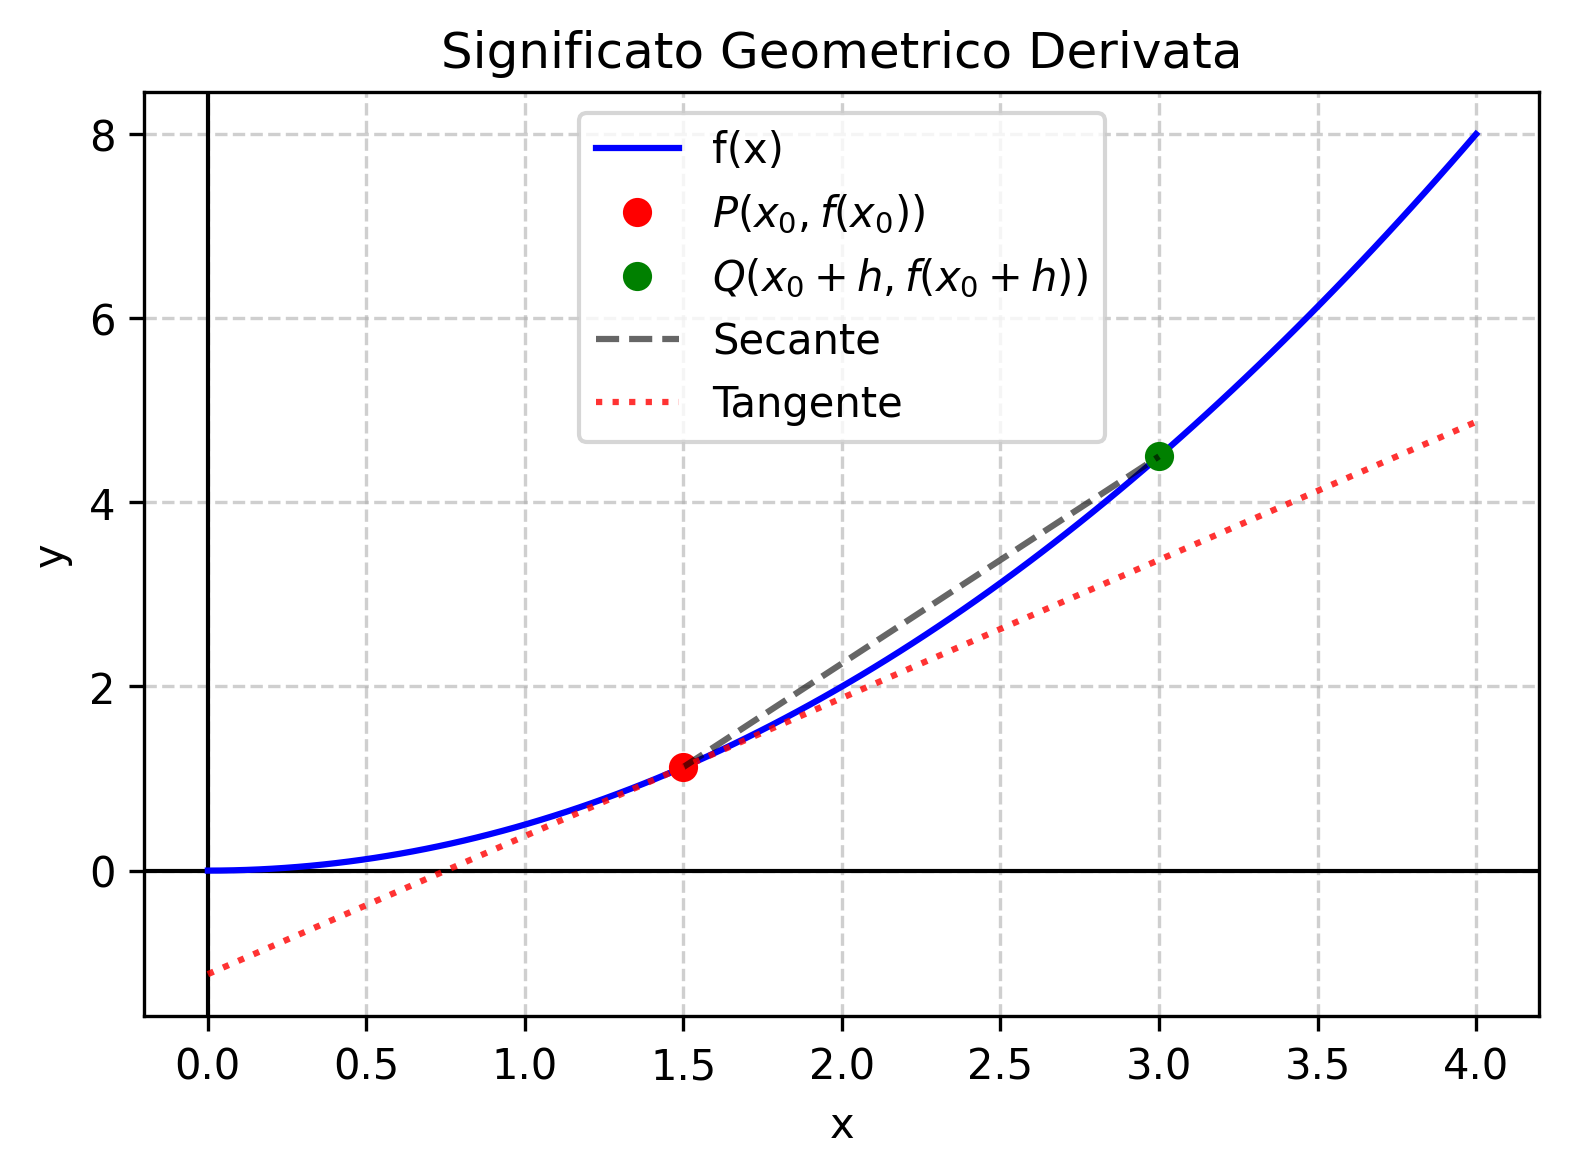
\includegraphics[width=0.7\textwidth]{img/rapporto_incrementale.png}
    \end{center}
    Prendiamo la secante passante per i punti \(P\) e \(Q\) e avviciniamoli (facendo tendere \(h \to 0\)).
    L'equazione della secante è:
    \[s: y=f(x_{0})+m(x-x_{0}) \quad \text{con } m=\frac{\Delta f}{\Delta x}\]
    
    Passaggio al limite:
    \begin{align*}
    &s: y=f(x_{0})+\frac{f(x_{0}+h)-f(x_{0})}{h}(x-x_{0})\\
    &h\to 0 \implies \\
    &\frac{f(x_{0}+h)-f(x_{0})}{h} \to l \\
    & s\to t:y=f(x_{0})+l(x-x_{0})
    \end{align*}
}

\subsection{Definizione di Derivata}

\defn{Derivata}{
    Si chiama \textbf{derivata} di \(f\) in \(x_{0}\) il seguente limite, se esiste finito:
    \[\lim_{ h \to 0 } \frac{f(x_{0}+h)-f(x_{0})}{h}=l\in \mathbb{R}\]
    Tale limite si denota con uno dei seguenti simboli:
    \begin{itemize}
        \item \(f'(x_{0})\)
        \item \(\frac{d}{dx}f(x_{0})\)
        \item \(Df(x_{0})\)
    \end{itemize}
    Se \(f\) ha derivata in \(x_{0}\), si dice \textbf{derivabile} in \(x_{0}\).
    Se \(f\) è derivabile \(\forall x_{0} \in ]a,b[\) diremo che \(f\) è derivabile.
}

\defn{Retta Tangente}{
    Se \(f\) è derivabile in \(x_{0}\), la retta
    \[y=f(x_{0})+f'(x_{0})(x-x_{0})\]
    prende il nome di \textbf{retta tangente} al grafico di \(f\) nel punto \((x_{0},f(x_{0}))\) e \(f'(x_{0})\) è il suo coefficiente angolare.
    
    Posso anche scrivere la derivata nella forma alternativa:
    \[f'(x_{0})=\lim_{ h \to 0 } \frac{f(\overbrace{x_{0}+h}^{x})-f(x_{0})}{h}=\lim_{ x \to x_{0} } \frac{f(x)-f(x_{0})}{x-x_{0}}\]
}

\subsection{Derivata Destra e Sinistra}

Se consideriamo una funzione definita su un intervallo chiuso o se vogliamo studiare la derivabilità agli estremi \(x_{0}=a\) o \(x_{0}=b\), definiamo:

\defn{Derivata Destra e Sinistra}{
    \begin{itemize}
        \item Se \(\lim_{ x \to x_{0}^+ } \frac{f(x)-f(x_{0})}{x-x_{0}} = l_+ \in \mathbb{R}\), allora lo indichiamo con \(f'_{+}(x_{0})\) e si chiama \textbf{derivata destra} in \(x_{0}\).
        \item Se \(\lim_{ x \to x_{0}^- } \frac{f(x)-f(x_{0})}{x-x_{0}} = l_- \in \mathbb{R}\), allora lo indichiamo con \(f'_{-}(x_{0})\) e si chiama \textbf{derivata sinistra} in \(x_{0}\).
    \end{itemize}
}

\rmkb{
    \(f\) è derivabile in \(x_{0} \iff f'_{+}(x_{0})\) e \(f'_{-}(x_{0})\) esistono finiti e coincidono:
    \[f'(x_{0})=f'_{+}(x_{0})=f'_{-}(x_{0})\]
}



\section{Derivate delle Funzioni Elementari}

Di seguito analizziamo le derivate delle funzioni fondamentali, dimostrandone i risultati tramite la definizione di rapporto incrementale.

\begin{enumerate}
    \item \textbf{Derivata di una costante} \(c\):
    \[ Dc(x)=0 \; \forall x\in \mathbb{R} \]
    Infatti: \(\lim_{ x \to x_{0} } \frac{c-c}{x-x_{0}}=0\).
    \begin{center}
        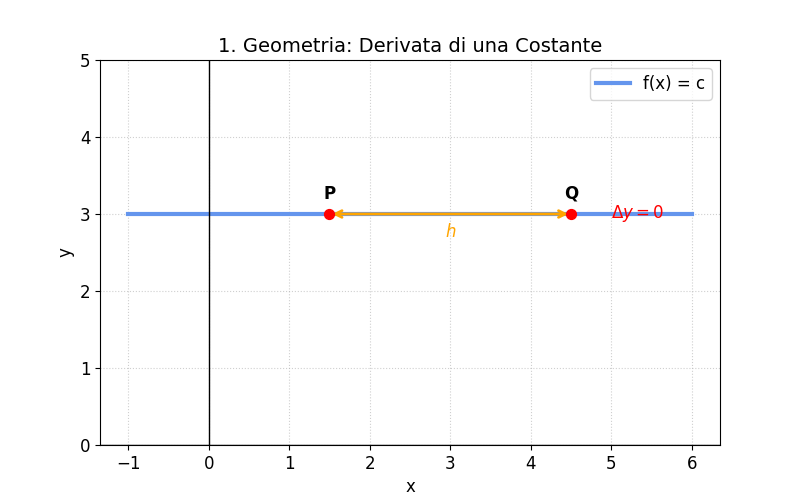
\includegraphics[width=0.6\textwidth]{img/der-di-costante.png}
    \end{center}

    \item \textbf{Derivata della retta} \(ax+b\):
    \[ D(ax+b)=\lim_{ h \to 0 } \frac{a(x+h)+b-ax-b}{h}=\lim_{ h \to 0 } \frac{ah}{h}=a \]
    \begin{center}
        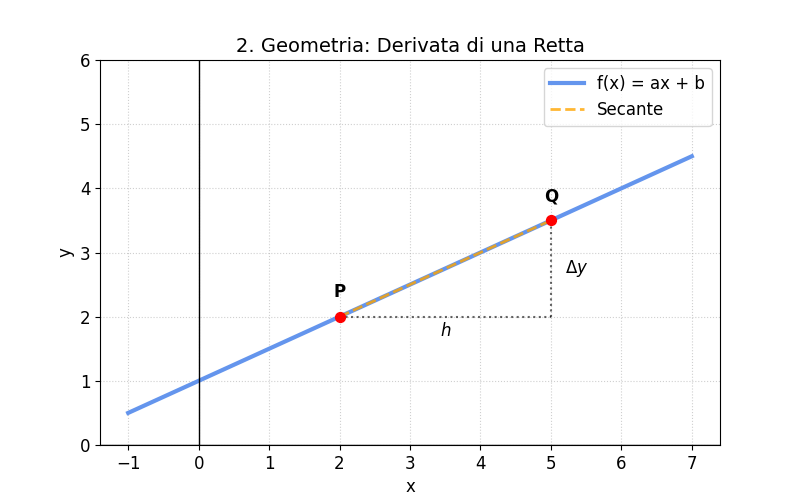
\includegraphics[width=0.6\textwidth]{img/der-di-retta.png}
    \end{center}
    \ex{
        \(D(x)=1\) \\
        \(D(-x)=-1\)
    }

    \item \textbf{Derivata del valore assoluto} \(|x|\):
    \[
    |x|=\begin{cases}
    x & x\geq 0 \\
    -x & x<0
    \end{cases} \implies
    D(|x|)=\begin{cases}
    1 & x>0 \\
    -1 & x<0 \\
    \not \exists & x=0
    \end{cases}
    \]
    Perché in \(x=0\):
    \[\lim_{ h \to 0 } \frac{|0+h|-|0|}{h}=\frac{|h|}{h}=\begin{cases} 1 & h \to 0^+ \\ -1 & h \to 0^- \end{cases} \implies \not \exists\]

    \item \textbf{Derivata della potenza} \(x^\alpha\):
    \[ D(x^\alpha)=\alpha x^{\alpha-1} \]
    \pf{
        \begin{align*}
        & \lim_{ h \to 0 } \frac{f(x+h)-f(x)}{h}=\lim_{ h \to 0 } \frac{(x+h)^\alpha-x^\alpha}{h}= \left[\frac{0}{0}\right] \\
        & = \lim_{ h \to 0 } \frac{x^\alpha \left( \left( 1+\frac{h}{x} \right)^\alpha-1 \right)}{h}=\lim_{ h \to 0 } \frac{x^{\alpha-1}\left( \left( 1+\frac{h}{x} \right)^\alpha-1 \right)}{\frac{h}{x}}=\alpha x^{\alpha-1}
        \end{align*}
    }
    \ex{
        \begin{itemize}
            \item \(D(\sqrt{ x }) = D(x^{1/2}) = \frac{1}{2}x^{\frac{1}{2} -1}=\frac{1}{2\sqrt{ x }}\)
            \item \(D(x^3)=3x^2\)
        \end{itemize}
    }

    \item \textbf{Derivata dell'esponenziale} \(a^x\):
    \[ D(a^x) = a^x \log a \]
    \pf{
        \[\lim_{ h \to 0 } \frac{a^{x+h}-a^x}{h}=\lim_{ h \to 0 } \frac{a^x(a^h-1)}{h} = a^x\log a\]
    }

    \item \textbf{Derivata di} \(e^x\):
    \[ D(e^x)=e^x \]
    (Segue dalla (5) ponendo \(a=e\), dato che \(\log e = 1\)).

    \item \textbf{Derivata del Seno}:
    \[ D(\sin x)=\cos x \]
    \pf{
        \begin{align*}
        &\lim_{ h \to 0 } \frac{\sin(x+h)-\sin x}{h}= \lim_{ h \to 0 } \frac{\sin x\cos h + \cos x \sin h - \sin x}{h}=\\
        & = \lim_{ h \to 0 } \left[ \sin x \left( \frac{\cos h-1}{h} \right) + \cos x\left( \frac{\sin h}{h} \right) \right] = \sin x \cdot 0 + \cos x \cdot 1 = \cos x
        \end{align*}
    }

    \item \textbf{Derivata del Coseno}:
    \[ D(\cos x)=-\sin x \]
    \pf{
        \begin{align*}
        &\lim_{ h \to 0 } \frac{\cos(x+h)-\cos x}{h}=\lim_{ h \to 0 } \frac{\cos x \cos h - \sin x \sin h - \cos x}{h}=\\
        & = \lim_{ h \to 0 } \left[ \cos x\frac{(\cos h-1)}{h} - \sin x \cdot \frac{\sin h}{h} \right] = -\sin x
        \end{align*}
    }

    \item \textbf{Derivata del Logaritmo} \(\log_a x\):
    \[ D(\log_{a}x) = \frac{1}{x \log a} \]
    \pf{
        \[\lim_{ h \to 0 } \frac{\log_{a}(x+h)-\log_{a}(x)}{h}=\lim_{ h \to 0 } \frac{1}{h} \log_{a}\left( 1+ \frac{h}{x} \right) = \lim_{ h \to 0 } \frac{1}{x} \frac{\log_{a}(1+t)}{t} = \frac{1}{x\log a}\]
        (dove \(t = h/x \to 0\)).
    }

    \item \textbf{Derivata di} \(\log x\) (base \(e\)):
    \[ D(\log x)=\frac{1}{x} \]

\end{enumerate}

\section{Algebra delle Derivate}

\thm{Operazioni con le Derivate}{
    Siano \(f, g\) definite in \(]a,b[\) e derivabili in \(x_{0}\). Allora anche \(c \cdot f\), \(f\pm g\), \(f \cdot g\) e \(\frac{f}{g}\) (se \(g(x_0)\neq 0\)) sono derivabili in \(x_{0}\) e risulta:
    \begin{enumerate}
        \item \(D(cf(x_{0}))=cDf(x_{0})\)
        \item \(D(f\pm g)(x_0)=Df(x_{0})\pm Dg(x_{0})\)
        \item \(D(fg)(x_{0})=Df(x_{0})g(x_{0})+f(x_{0})Dg(x_{0})\)
        \item \(D\left( \frac{f}{g} \right)(x_{0})=\frac{Df(x_{0})g(x_{0})-f(x_{0})Dg(x_{0})}{g^2(x_{0})}\)
    \end{enumerate}
    Le proprietà (1) e (2) indicano che la derivata è un \textbf{operatore lineare}.
}

\pf{
    \textbf{Dimostrazione (2) - Somma:}
    \[\lim_{ h \to 0 } \frac{f(x_{0}+h)+g(x_{0}+h)-(f(x_{0})+g(x_{0}))}{h}= \]
    \[=\lim_{ h \to 0 } \left[ \frac{f(x_0+h)-f(x_0)}{h} + \frac{g(x_0+h)-g(x_0)}{h} \right]=\]
    \[= f'(x_{0})+g'(x_{0})\]
}

Per dimostrare rigorosamente la regola del prodotto, necessitiamo prima di un legame tra derivabilità e continuità.

\thm{Relazione Derivabilità-Continuità}{
    Se \(g\) è definita in \(]a,b[\) ed è derivabile in \(x_{0} \implies g\) è continua in \(x_{0}\).
    
    Il viceversa non vale: \(\centernot \impliedby\). Esempio: \(|x|\) è continua in \(x=0\) ma non derivabile.
}

\pf{
    Per dimostrare che \(g\) è continua in \(x_{0}\) devo dimostrare che \(\lim_{ x \to x_{0} } g(x)=g(x_{0})\), ovvero che \(\lim_{ x \to x_{0} } (g(x)-g(x_{0}))=0\).
    Possiamo scrivere:
    \[\lim_{ x \to x_{0} } (g(x)-g(x_{0})) = \lim_{ x \to x_{0} } \frac{g(x)-g(x_{0})}{x-x_{0}}(x-x_{0}) = g'(x_0) \cdot 0 = 0\]
}

\pf{
    \textbf{Dimostrazione (3) - Prodotto:}
    \begin{align*}
    &\lim_{ x \to x_{0} } \frac{f(x)g(x)-f(x_{0})g(x_{0})}{x-x_{0}} \\ 
    &= \lim_{ x \to x_{0} } \frac{f(x)g(x) - f(x_0)g(x) + f(x_0)g(x) - f(x_0)g(x_0)}{x-x_{0}} \\ 
    &= \lim_{ x \to x_{0} } \left( g(x) \frac{f(x)-f(x_0)}{x-x_0} + f(x_0) \frac{g(x)-g(x_0)}{x-x_0} \right) \\ 
    &= g(x_0)f'(x_0) + f(x_0)g'(x_0) 
    \end{align*}
    (Qui abbiamo usato il fatto che \(\lim_{x \to x_0} g(x) = g(x_0)\) perché \(g\) è derivabile e quindi continua).
}

\ex{
    \textbf{Derivata della Tangente}:
    \begin{align*}
    & D(\tan x) = D\left(\frac{\sin x}{\cos x} \right)=\frac{\cos x \cdot \cos x - \sin x (-\sin x)}{\cos^2 x} = \\
    &\frac{\cos^2 x + \sin^2 x}{\cos^2 x} = \\
    & \frac{1}{\cos^{2}x} = 1+\tan^2 x
    \end{align*}
}

\section{Teoremi Fondamentali del Calcolo}

\thm{Derivazione delle Funzioni Composte (Chain Rule)}{
    Siano \(g,f\) tali che sia definita la funzione composta \(f(g(x))\).
    Sia \(x_{0}\) tale che \(g\) è derivabile in \(x_{0}\) e \(f\) è derivabile in \(g(x_{0})\).
    Allora \(f \circ g\) è derivabile in \(x_{0}\) e si ha:
    \[D(f \circ g)(x)=(f \circ g)'(x_{0})=f'(g(x_{0}))\cdot g'(x_{0})\]
}

\pf{
    Definiamo la funzione ausiliaria \(H(y)\):
    \[H(y)=\begin{cases}
    \frac{f(y)-f(y_{0})}{y-y_{0}} & y\ne y_0\\
    f'(y_{0}) & y=y_{0}
    \end{cases}\]
    dove \(y_0 = g(x_0)\). \(H\) è continua in \(y_{0}\).
    Possiamo scrivere il rapporto incrementale come:
    \[\frac{f(g(x))-f(g(x_{0}))}{x-x_{0}} = H(g(x))\frac{g(x)-g(x_{0})}{x-x_{0}}\]
    Passando al limite per \(x \to x_0\):
    \[\lim_{ x \to x_{0} } H(g(x))\frac{g(x)-g(x_{0})}{x-x_{0}} = H(g(x_0)) \cdot g'(x_0) = f'(g(x_{0}))\cdot g'(x_{0})\]
}

\thm{Derivata della Funzione Inversa}{
    Sia \(f\) strettamente monotona e continua in \(]a,b[\).
    Sia \(f\) derivabile in \(x_{0}\in]a,b[\) e \(f'(x_{0})\neq 0\).
    Allora la funzione inversa \(f^{-1}\) è derivabile in \(y_{0}=f(x_{0})\) e risulta:
    \[(f^{-1})'(y_{0})=\frac{1}{f'(f^{-1}(y_{0}))}=\frac{1}{f'(x_{0})}\]
}

\begin{center}
    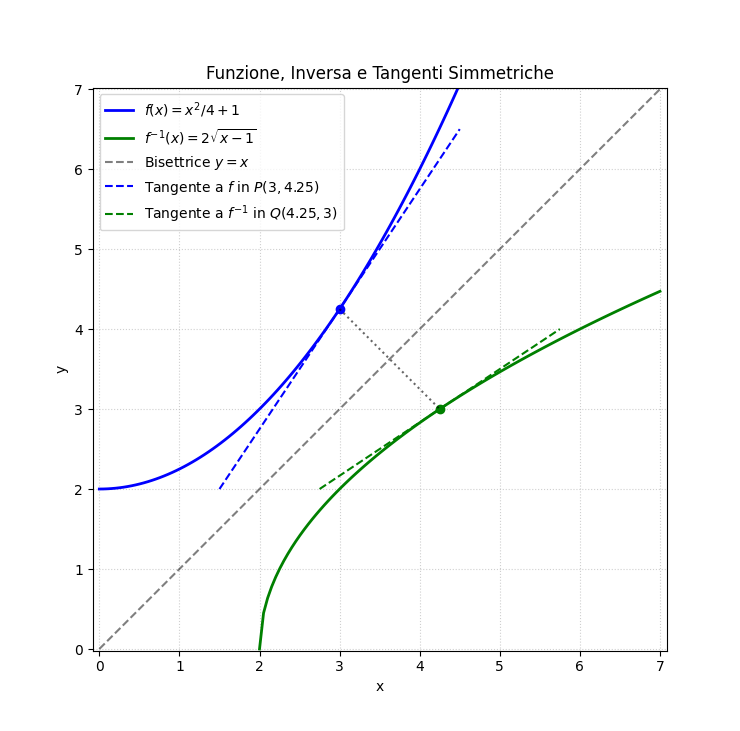
\includegraphics[width=0.6\textwidth]{img/derivata_funzione_inversa.png}
\end{center}

\rmkb{
    Interpretazione geometrica: Se la retta tangente in \(P(x_0, y_0)\) forma un angolo \(\alpha\) con l'asse \(x\), allora \(f'(x_0) = \tan \alpha\). Rispetto all'asse \(y\) (scambiando gli assi per l'inversa), l'angolo è \(\beta = \frac{\pi}{2} - \alpha\).
    \[(f^{-1})'(y_{0})=\tan \beta = \tan\left( \frac{\pi}{2} -\alpha \right)=\frac{1}{\tan \alpha}=\frac{1}{f'(x_{0})}\]
}

\subsection{Derivate delle Funzioni Inverse Trigonometriche}

\ex{
    \textbf{Arcoseno}:
    \[D(\arcsin x)=\frac{1}{D(\sin y)}\bigg|_{y=\arcsin x}=\frac{1}{\cos y}\]
    Poiché \(y \in [-\frac{\pi}{2}, \frac{\pi}{2}]\), \(\cos y \ge 0\), quindi \(\cos y = \sqrt{1-\sin^2 y}\).
    \[= \frac{1}{\sqrt{ 1-\sin^2 (\arcsin x) }} = \frac{1}{\sqrt{ 1-x^2 }}\]
}

\ex{
    \textbf{Arcocoseno}:
    \[D(\arccos x) = \frac{1}{D(\cos y)}\bigg|_{y=\arccos x} = \frac{1}{-\sin y}\]
    Poiché \(y \in [0, \pi]\), \(\sin y \ge 0\), quindi \(\sin y = \sqrt{1-\cos^2 y}\).
    \[= -\frac{1}{\sqrt{1-x^2}}\]
}

\ex{
    \textbf{Arcotangente}:
    \[D(\arctan x) = \frac{1}{D(\tan y)}\bigg|_{y=\arctan x} = \cos^2 y = \frac{1}{1+\tan^2 y} = \frac{1}{1+x^2}\]
}


\section{Punti di non derivabilità}\label{punti-di-non-derivabilituxe0}

% Utilizzo dell'ambiente \defn definito in theorems.tex
% Argomento 1: Titolo (opzionale o desunto dal testo)
% Argomento 2: Contenuto
\defn{\(f\) non derivabile}{
    Se \(f\) non è derivabile in \(x_{0}\):
    \[
    \lim_{ x \to x_{0} } \frac{f(x)-f(x_{0})}{x-x_{0}}=\begin{cases}
    \not \exists \\ 
    \infty
    \end{cases}
    \]
}

\begin{enumerate}
    \item \(f'_{+}(x_{0})\) e \(f'_{-}(x_{0}) \exists\) finite ma:
    \[f'_{+}(x_{0})\neq f'_{-}(x_{0})\] 
    In questo caso si chiama \textbf{punto angoloso}. Assumiamo che \(x_{0}\) è un punto angoloso anche quando una delle due derivate \(f'_{+}(x_{0})\) e \(f'_{-}(x_{0})\) è finita, mentre l'altra è \(\pm \infty\).
\end{enumerate}


\ex{
    \[
    f(x)=\begin{cases}
    \sqrt{ x } & x\geq{0} \\
    1- e^{-x/2} & x<0 
    \end{cases}
    \implies f\text{ è continua in } \mathbb{R}
    \]
    \[f'_{+}(0)= +\infty \qquad f'_{-}(0)=-\frac{1}{2}\]
    \begin{center}
    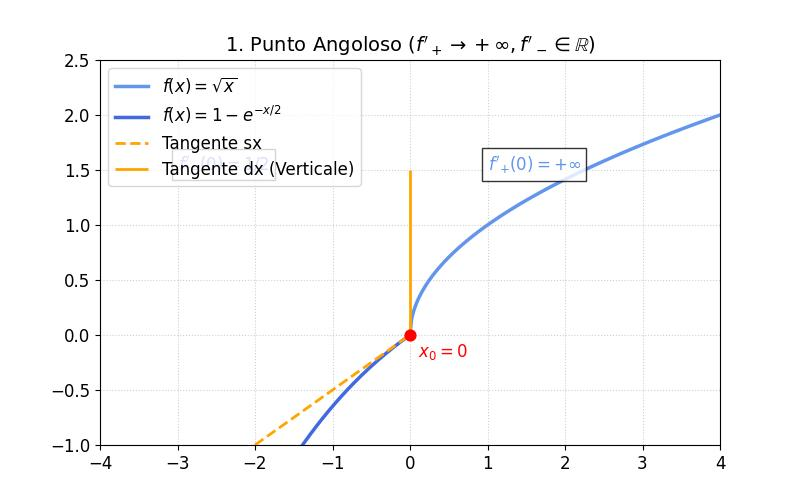
\includegraphics[width=0.7\textwidth]{img/punto_angoloso.png}
    \end{center}
}

\begin{enumerate}
    \setcounter{enumi}{1}
    \item Se \(f'_{+}(x_{0})=+\infty\) e \(f'_{-}(x_{0})=-\infty\) o viceversa, \(x_{0}\) si dice \textbf{cuspide}.
\end{enumerate}

\ex{
    \[ f(x)=\sqrt{ |x| } \]
    \begin{center}
    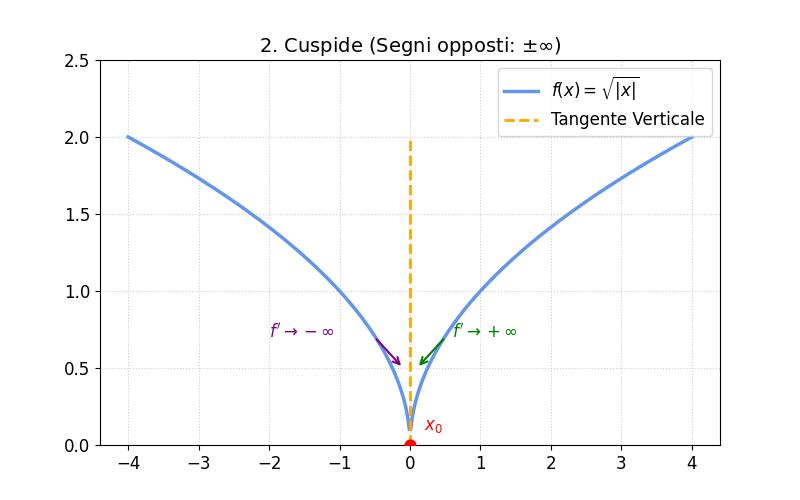
\includegraphics[width=0.7\textwidth]{img/cuspide.png}
    \end{center}
}

\begin{enumerate}
    \setcounter{enumi}{2}
    \item Se \(f'_{+}(x_{0})=f'_{-}(x_{0})=\pm \infty\) (\(\infty\) ma con lo stesso segno), \(x_{0}\) è \textbf{a tangente verticale.}
\end{enumerate}

\ex{
    \[ y=\sqrt[3]{x} \]
    \begin{center}
    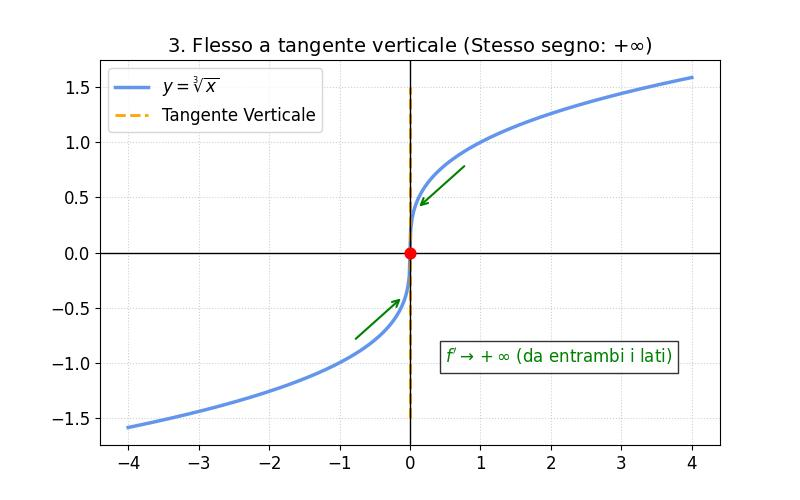
\includegraphics[width=0.7\textwidth]{img/flesso-tan-ver.png}
    \end{center}
}

Tutti gli altri sono punti di non derivabilità.

\rmkb{
    Le funzioni con derivata limitata sono sempre Lipschitziane.
}



\section{Estremi relativi}

\defn{Min relativo e punto di Min relativo}{
    Sia $f:A \subseteq \mathbb{R}\to \mathbb{R}, \quad A\neq \emptyset$.
    Un punto $x_{0}\in A$ si dice punto di minimo relativo per $f$ se $\exists I_{\delta}(x_{0})=]x_{0}-\delta,x_{0}+\delta[$ tale che:
    \[
    f(x)\geq f(x_{0}) \; \forall x \in A \cap I_{\delta}(x_{0})
    \]
    e $f(x_{0})$ si dice minimo relativo.
}

\defn{Max relativo e punto di Max relativo}{
    Se $\exists I_{\delta}(x_{0})=]x_{0}-\delta,x_{0}+\delta[$ tale che:
    \[
    f(x_{0})\geq f(x) \; \forall x \in A \cap I_{\delta}(x_{0})
    \]
    allora $x_{0}$ si dirà punto di massimo relativo e $f(x_{0})$ massimo relativo.
}

\ex{
    \begin{center}
        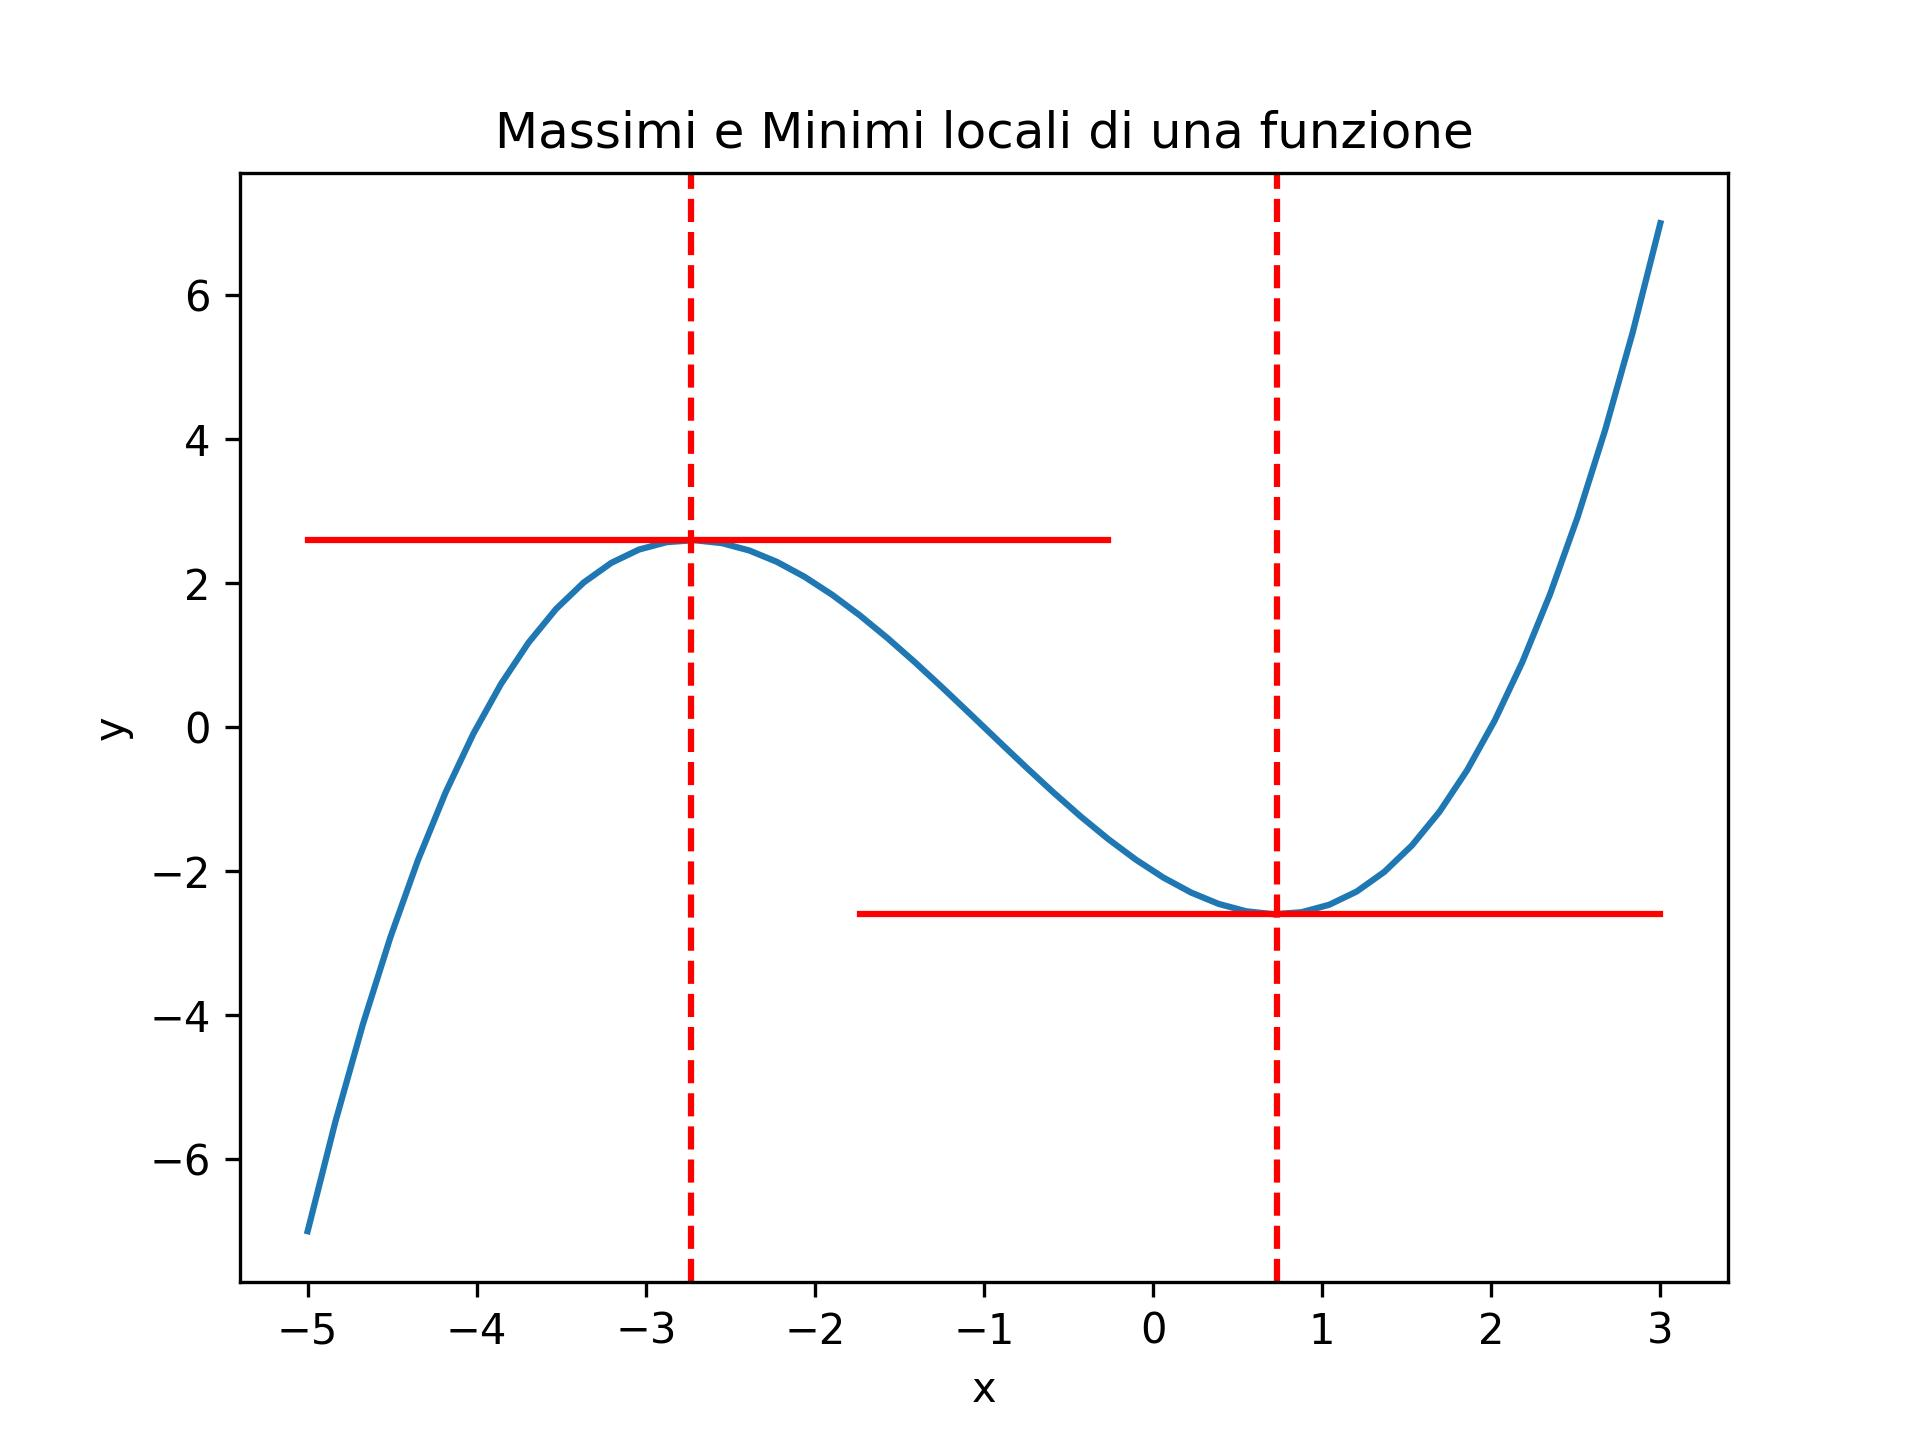
\includegraphics[width=0.7\textwidth]{img/estremi-relativi.jpg}
    \end{center}
}

\rmkb{NON SONO UNICI}

\subsection{Teorema di Fermat}

\thm{Teorema di Fermat (condizione necessaria del $1^{\circ}$ ordine)}{
    Sia $f:[a,b]\to \mathbb{R}$ e sia $x_{0}\in]a,b[$ un punto in cui $f$ è derivabile ed in un punto di estremo relativo.
    Allora ($\implies$):
    \[
    f'(x_{0})=0
    \]
}

\ex{
    \begin{center}
        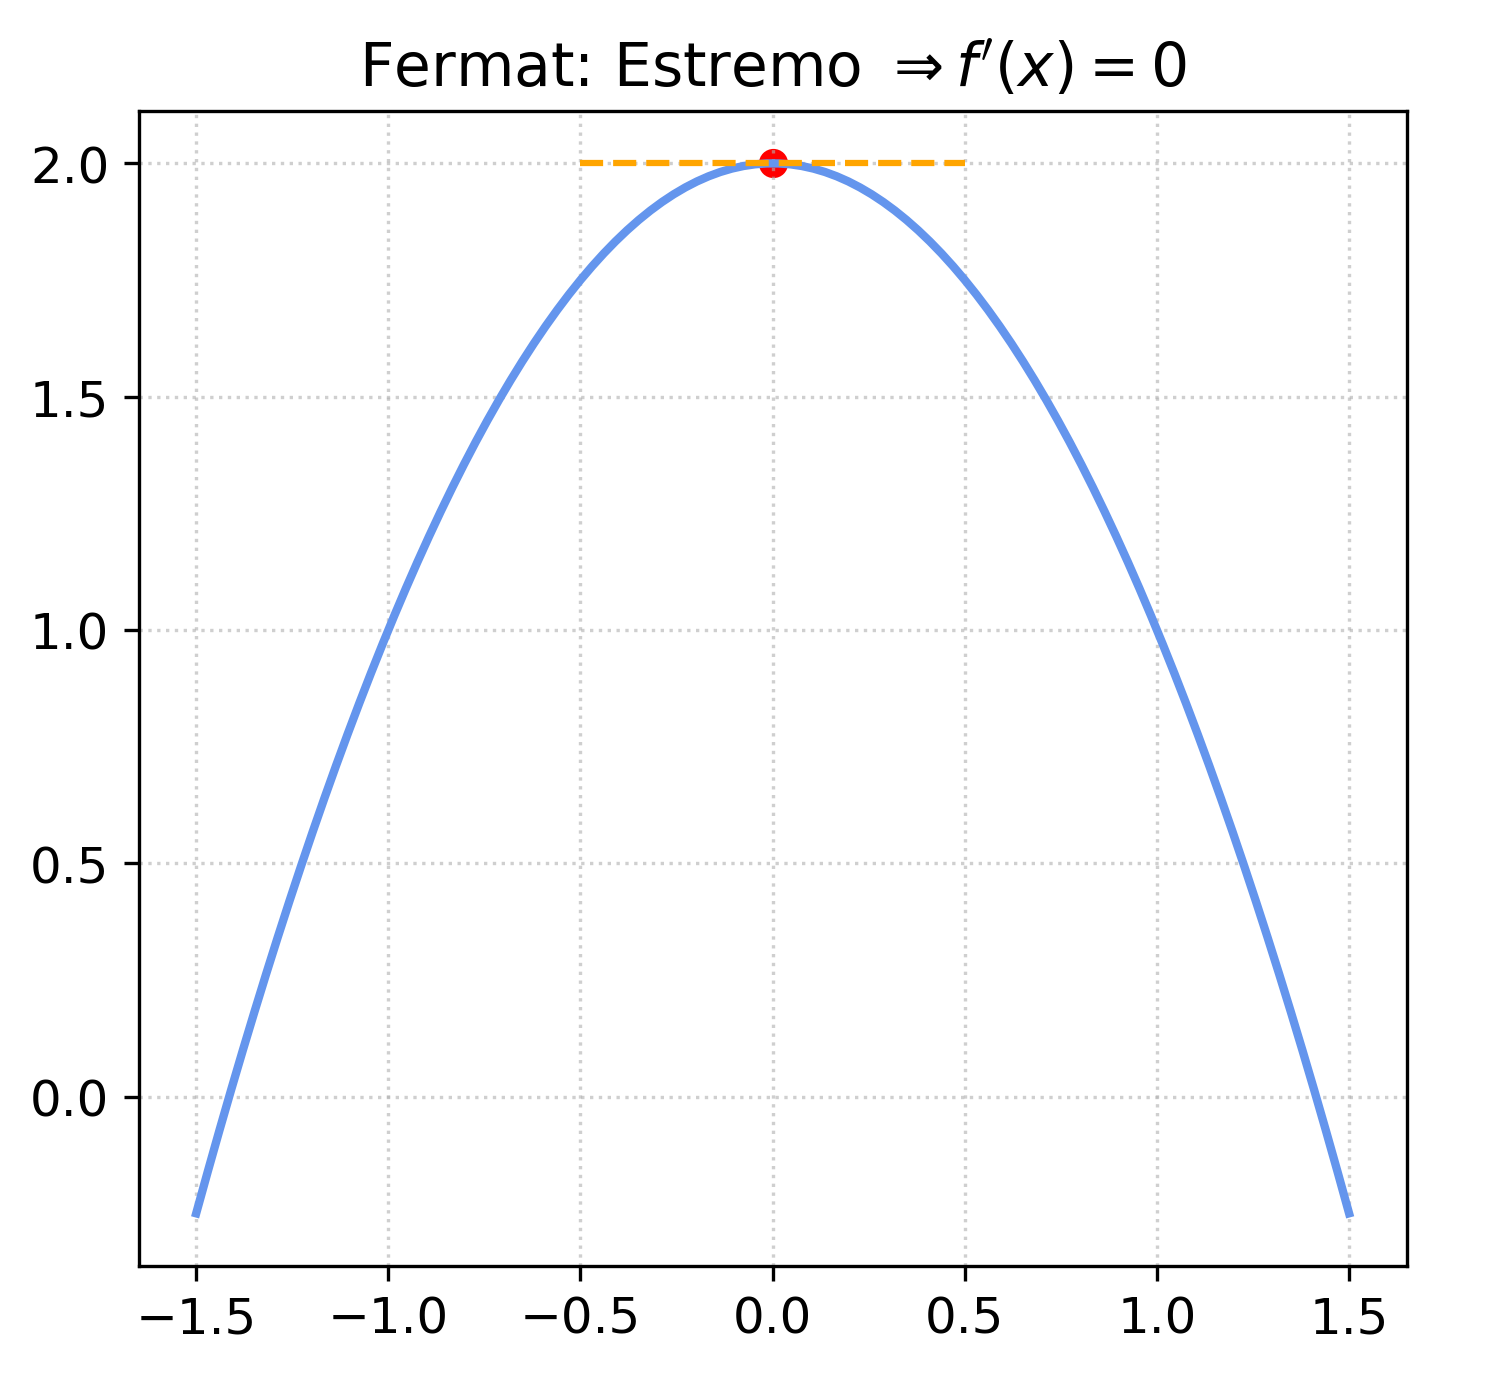
\includegraphics[width=0.7\textwidth]{img/teorema_fermat_es.png}
    \end{center}
}

\ex{
    Vale $\impliedby$? NO
    \begin{itemize}
        \item $\centernot \impliedby$
    \end{itemize}
    $f(x)=x^3 \quad f'(x)=3x^2$
    \begin{center}
        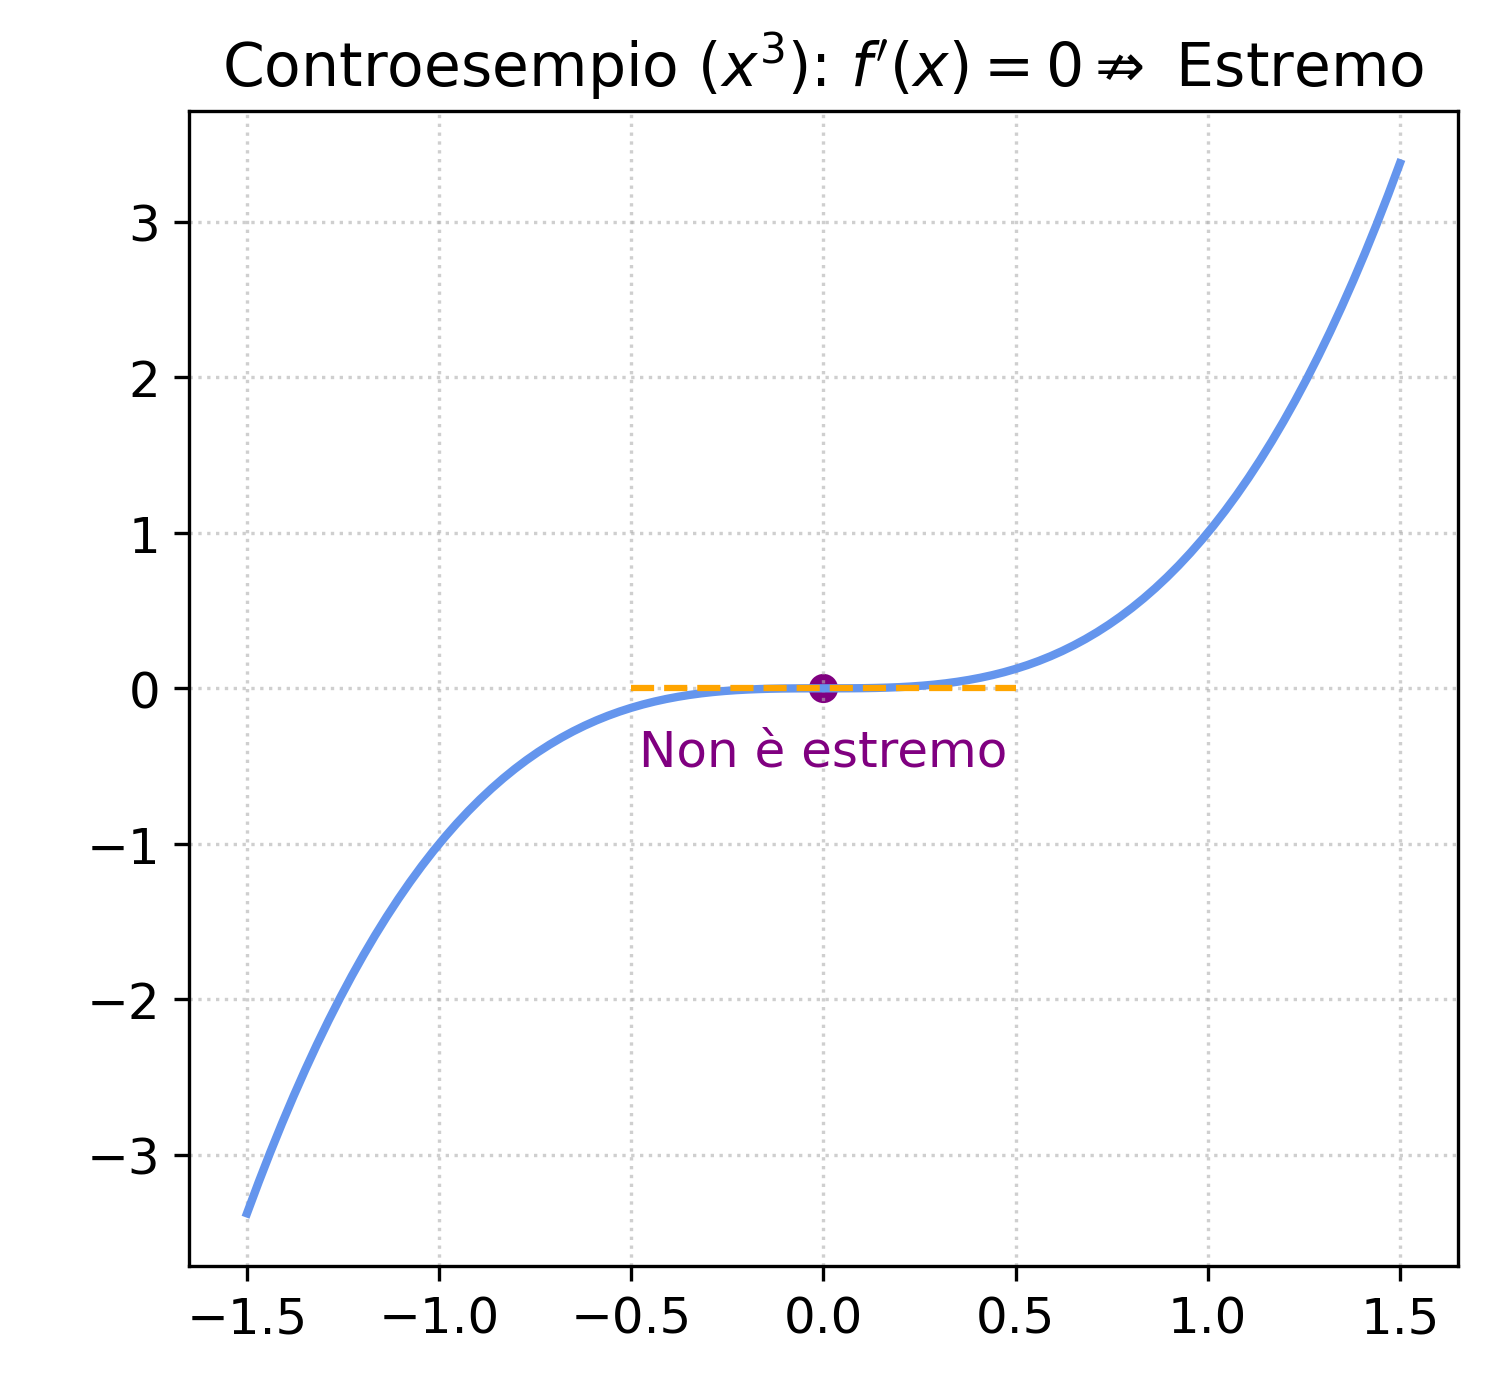
\includegraphics[width=0.7\textwidth]{img/teorema_fermat_controes.png}
    \end{center}
}

\pf{
    Supponiamo per semplicità che $x_{0}$ sia punto di minimo relativo, $\exists I_{\delta}(x_{0}):$
    \[
    f(x_{0})\leq f(x) \; \forall x \in [a,b] \cap I_{\delta}(x_{0})
    \]
    Essendo $f$ derivabile in $x_{0}$ allora:
    \begin{align*}
    \exists \text{ finito } &\lim_{ x \to x_{0} } \frac{f(x)-f(x_{0})}{x-x_{0}}=f'(x_{0}) \textcolor{orange}{=0}\\
    & =\lim_{ x \to x_{0}^- } \frac{f(x)-f(x_{0})}{x-x_{0}}=f'_{-}(x_{0}) \textcolor{orange}{\leq0}\\
    & =\lim_{ x \to x_{0}^+ } \frac{f(x)-f(x_{0})}{x-x_{0}}=f'_{+}(x_{0}) \textcolor{orange}{\geq0} 
    \end{align*}
    Il Numeratore è sempre positivo perchè nel limite, $x$ entra in $I_{\delta}(x_{0})$.
    Il segno del Denominatore dipende dal lato da cui avvicino, allora per avere l'uguaglianza, devono essere tutte (le derivate) = 0.
}

\defn{Definizione}{
    Sia $f$ derivabile in $]a,b[$, i punti $x: f'(x) = 0$.
    Si dicono \textbf{punti critici o stazionari}.
}

\subsubsection*{Esempio di esercizio}

\ex{
    \[ f(x)=2-\log(1+|x|) \qquad x\in[-1,3] \]
    Uso Weierstrass: $\exists$ estremi assoluti.
    Lista:
    \begin{enumerate}
        \item "Punti di Fermat"
        \item Punti di non Derivabilità
        \item Estremi
    \end{enumerate}
    
    \[
    f(x)= \begin{dcases}
    2-\log(1+x) \quad x\in[0,3] \\
    2-\log(1-x) \quad x \in[-1,0]
    \end{dcases}
    \]
    \[
    f'(x)= \begin{dcases}
    -\frac{1}{(1+x)} \quad x\in]0,3] \\
    \not \exists  \quad \qquad \qquad x=0\\
    \frac{1}{(1+x)} \quad x \in[-1,0[
    \end{dcases}\implies\text{Punto angoloso}
    \]
    \[ f(0)=2=M \qquad f(3)=2-\log_{4}=m \qquad f(-1)=2-\log_{2} \]
    
    Svolgimento lista:
    \begin{enumerate}
        \item $\to\varnothing$
        \item $\to x=0$
        \item $\to x=-1 \quad x=3$
    \end{enumerate}
}

\subsection{Teorema di Rolle}

\thm{Teorema di Rolle}{
    \begin{itemize}
        \item Sia $f:[a,b]\to \mathbb{R}$ continua
        \item Sia $f$ derivabile in $]a,b[$
        \item Se $f(a)=f(b)$ allora $\exists c \in ]a,b[:f'(c)=0$
    \end{itemize}
}

\ex{
    \begin{center}
        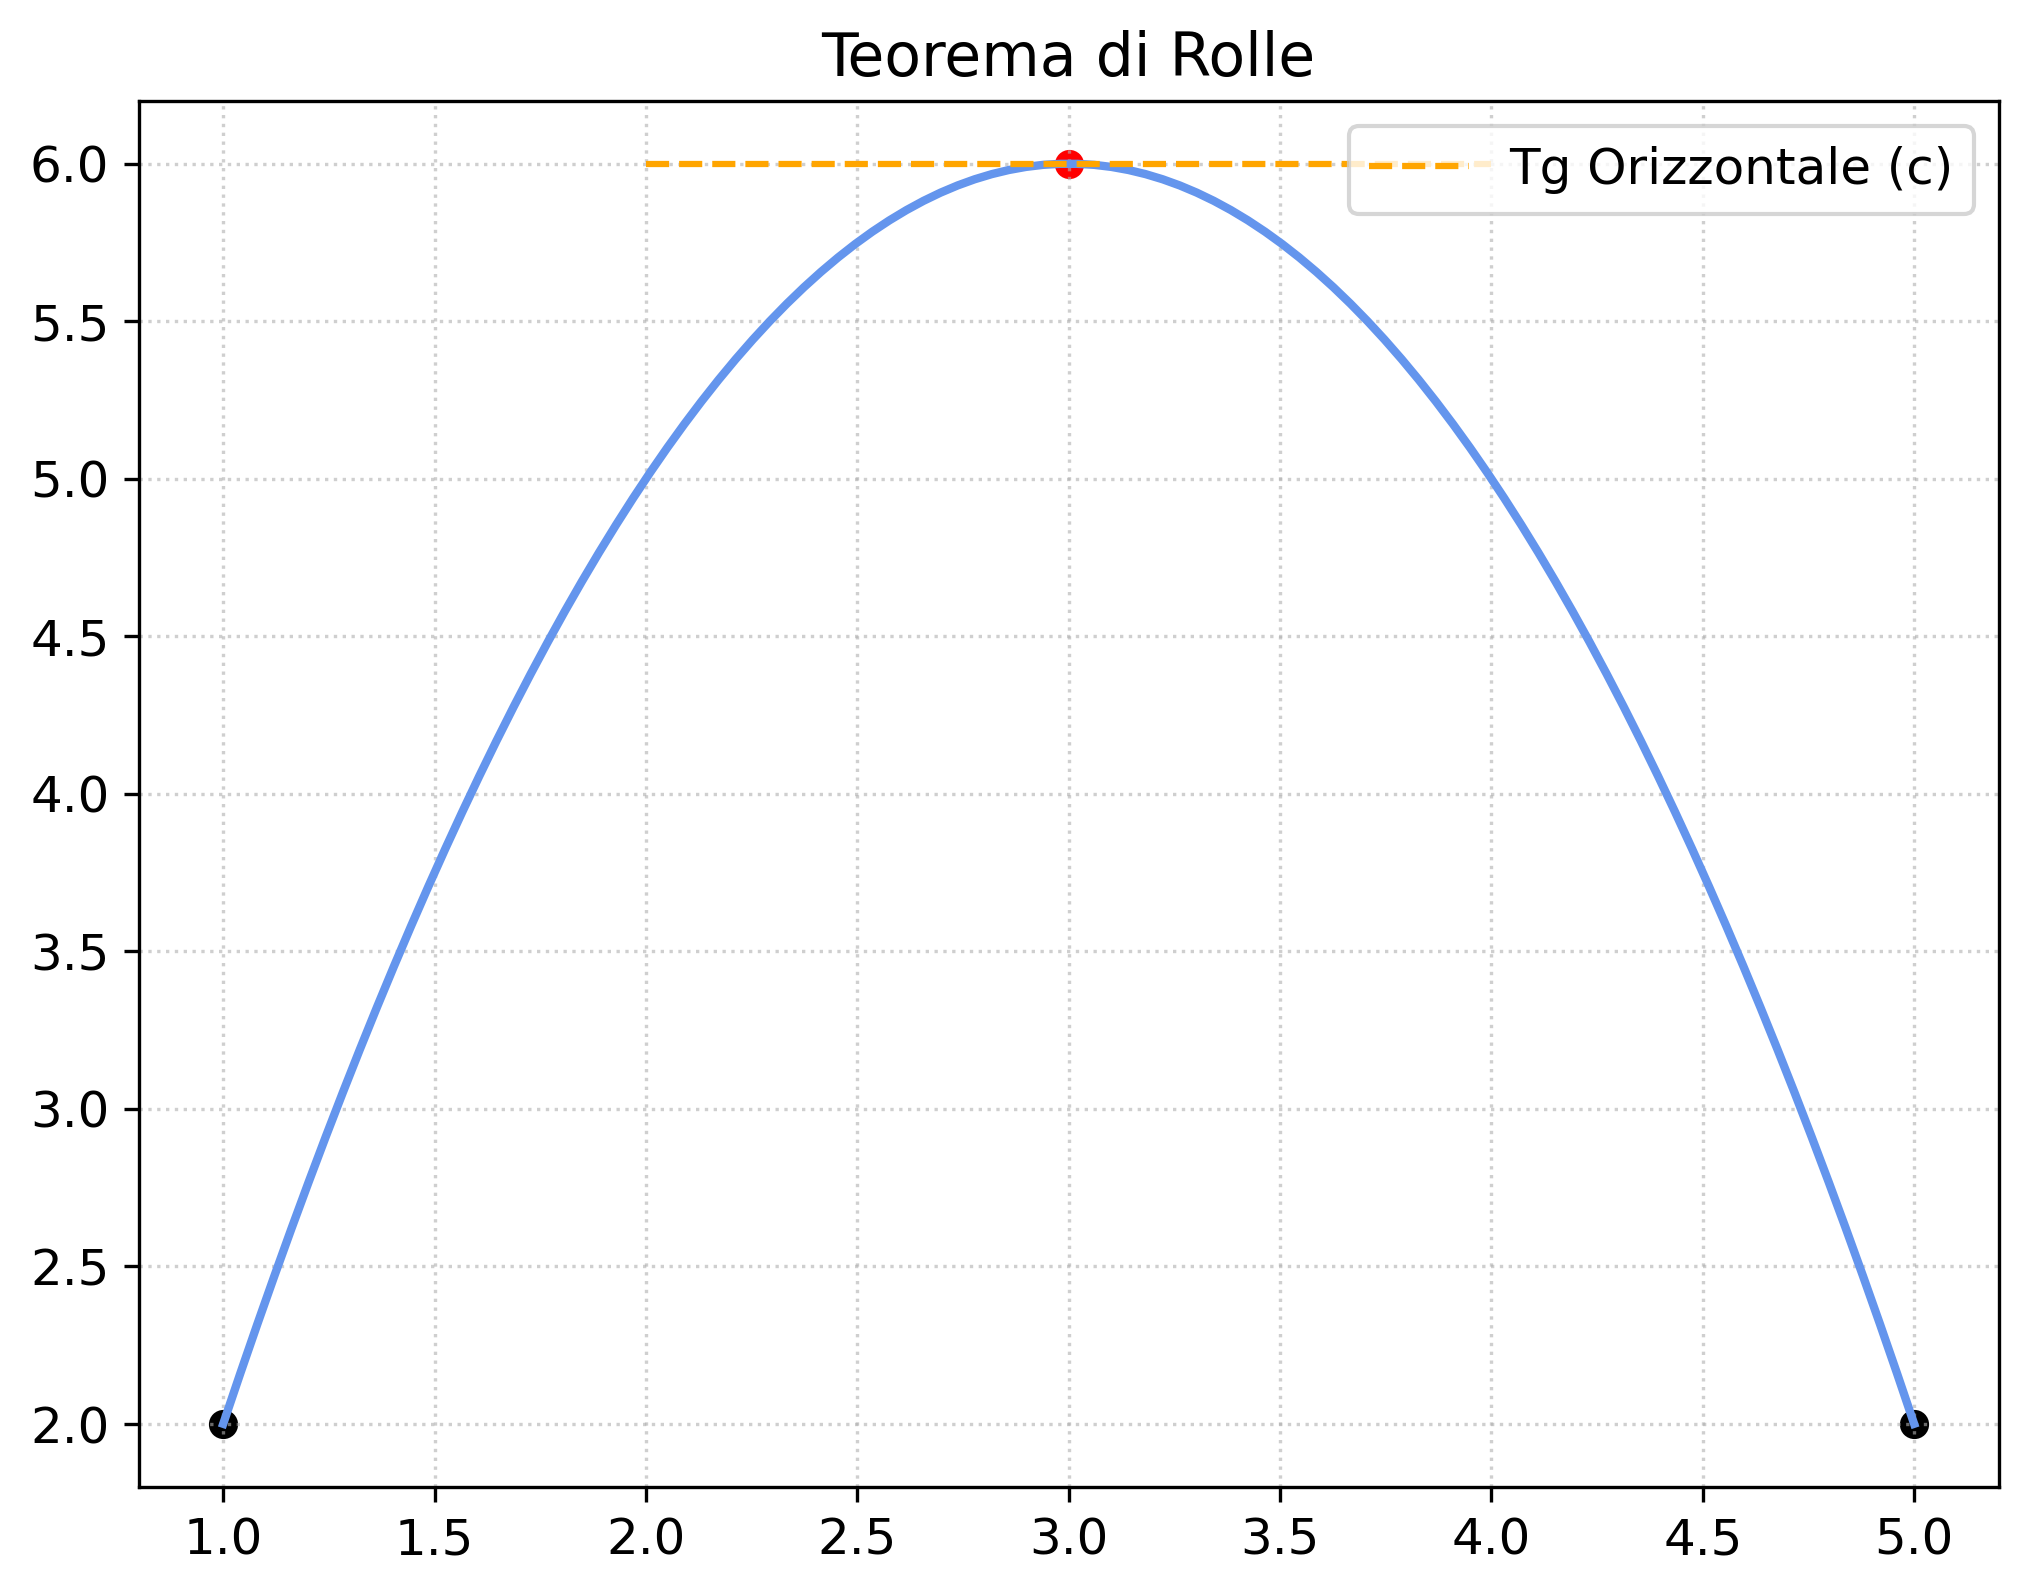
\includegraphics[width=0.7\textwidth]{img/teorema_rolle.png}
    \end{center}
}

\ex{
    Non posso rimuovere la prima ipotesi
    \begin{center}
        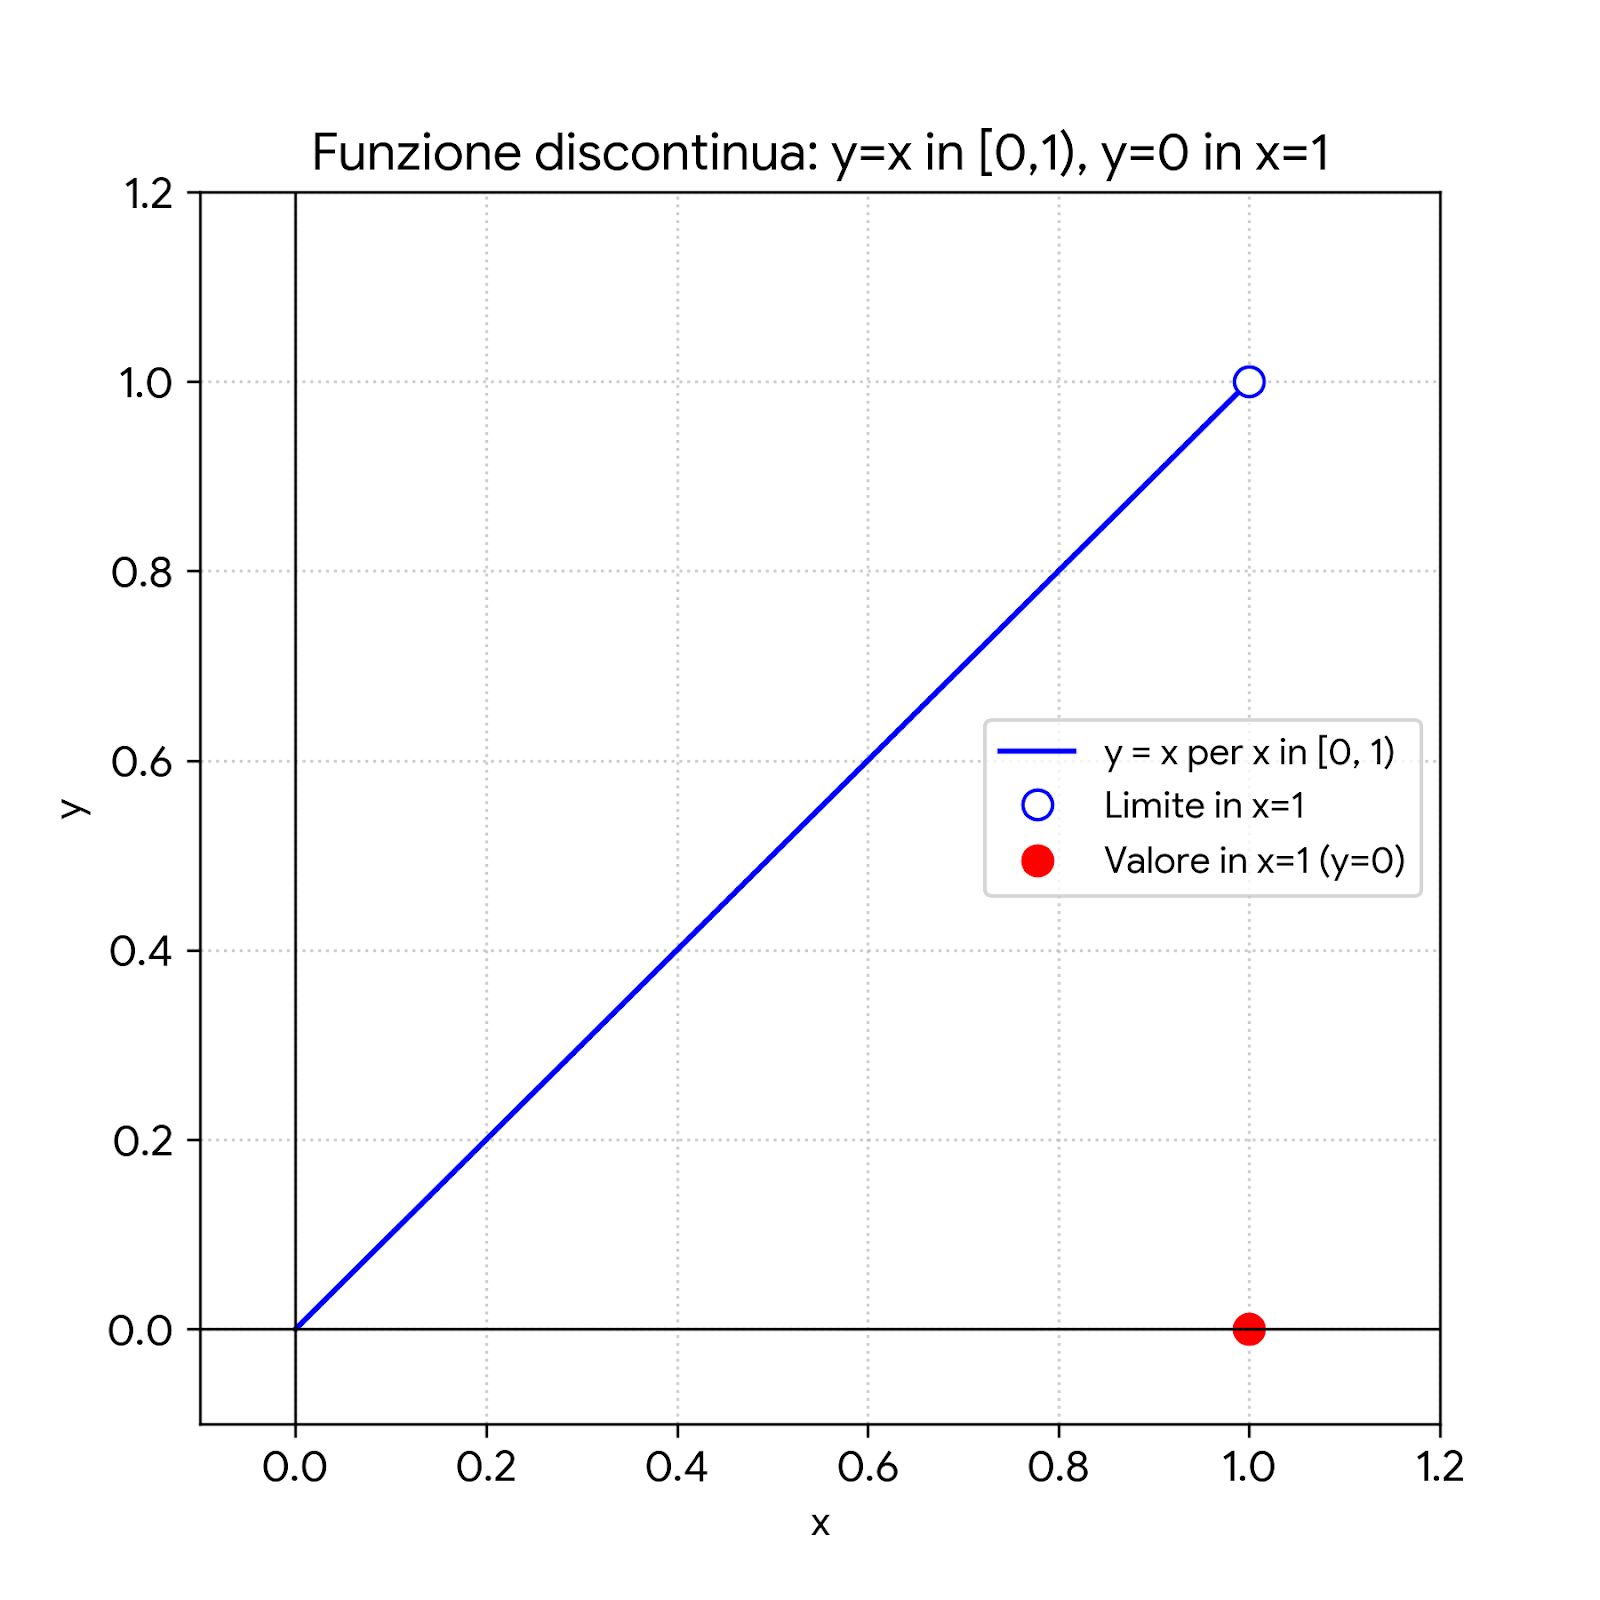
\includegraphics[width=0.7\textwidth]{img/percentuale-2.png}
    \end{center}
}

\pf{
    $\exists m = f(x_{m})$ e $M=f(x_{M})$ per Weierstrass con $x_{m}\in[a,b], x_{M}\in[a,b]$.
    Ovviamente $x_{m}\neq x_{M}$ altrimenti $f$ è costante:
    $m=M$ e in tal caso $\forall c \in [a,b] \implies f'(c)=0$.
    Ma se $x_{m}\neq x_{M}$ allora essendo per hp $f(a)=f(b)$ almeno uno dei 2 punti tra $x_{m}$ e $x_{M}$ deve essere interno ad $]a,b[$.
    Supponiamo che sia $x_{m}\in]a,b[\implies$ per Fermat $f'(x_{m})=0$.
}

\subsection{Teorema di Lagrange}

\thm{Teorema di Lagrange}{
    \begin{itemize}
        \item Sia $f:[a,b]\to \mathbb{R}$ continua 
        \item Sia $f$ derivabile in $]a,b[$
        \item Allora $\exists c \in]a,b[:$
        \[ m=f'(c)=\frac{f(b)-f(a)}{b-a} \]
    \end{itemize}
}

\ex{
    \begin{center}
        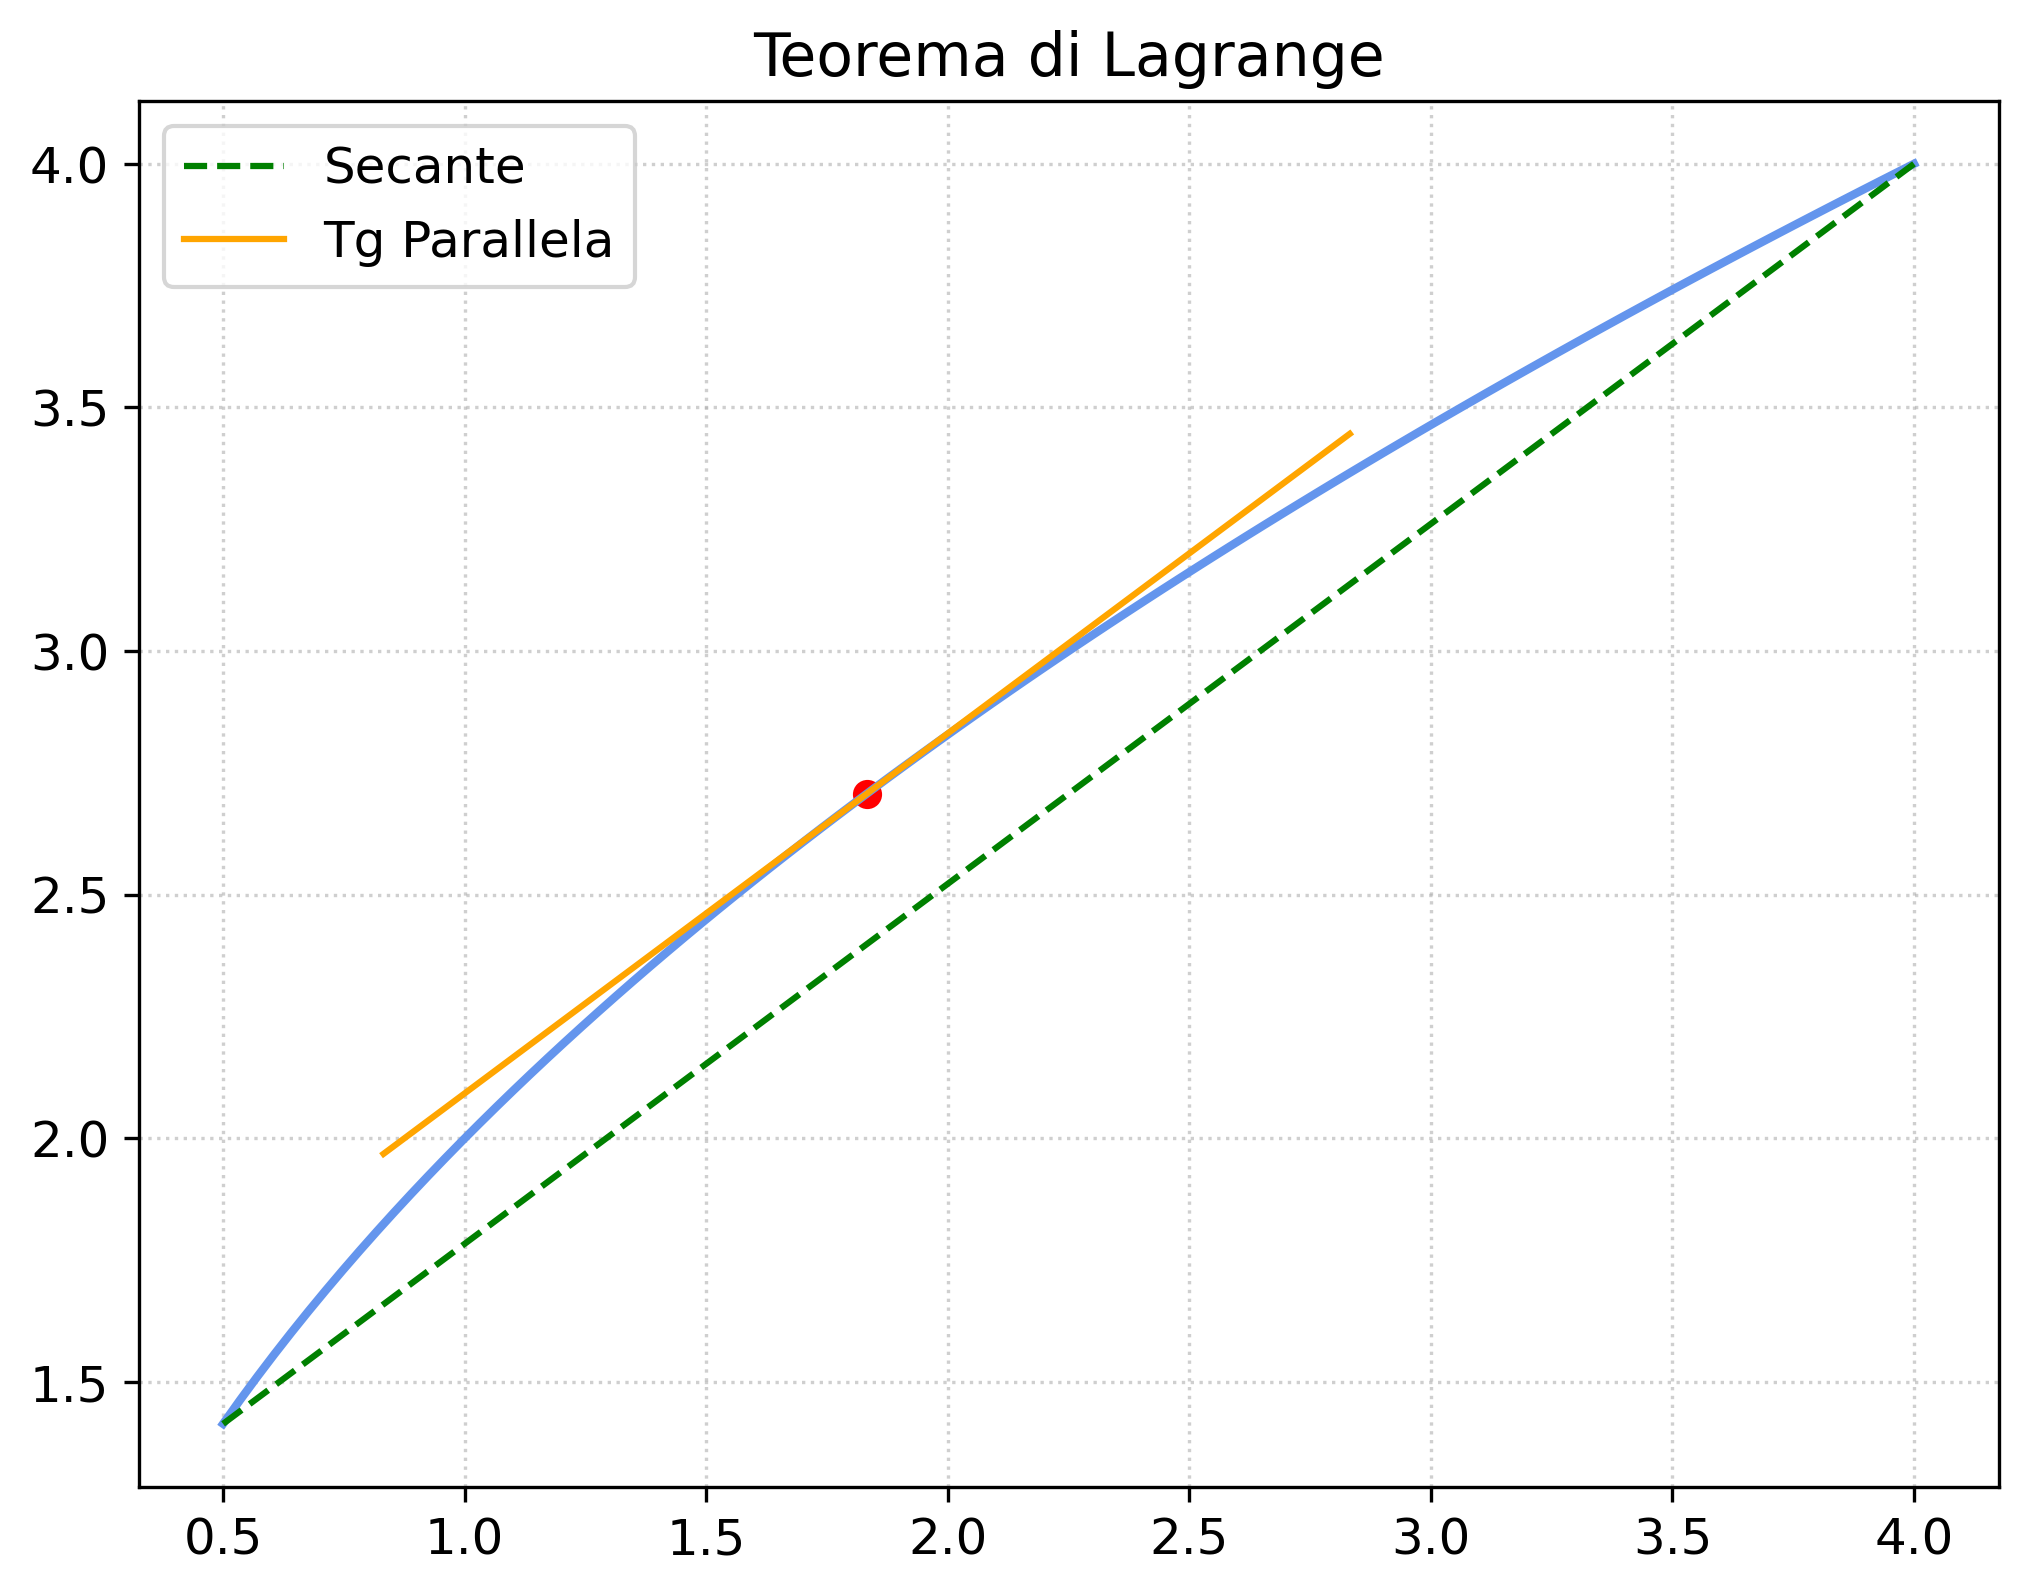
\includegraphics[width=0.7\textwidth]{img/teorema_lagrange.png}
    \end{center}
}

\pf{
    Consideriamo
    \[ g(x)=f(x)-\frac{f(b)-f(a)}{b-a}(x-a) \]
    \begin{itemize}
        \item $g$ è continua in $[a,b]$ (perchè è somma di funzioni continue)
        \item $g$ è derivabile in $]a,b[$
        \item $\begin{dcases}g(a)=f(a) \\ g(b)=f(a)\end{dcases}\implies \exists c \in]a,b[: g'(c)=0\implies$
    \end{itemize}
    \[ \implies f'(c)-\frac{f(b)-f(a)}{b-a}=0 \]
}

\subsubsection{Conseguenze del Teorema di Lagrange}

\thm{Teorema di Caratterizzazione delle funzioni costanti}{
    \begin{itemize}
        \item Sia $f$ continua in $[a,b]$
        \item Sia $f$ derivabile in $]a,b[$
    \end{itemize}
    \[ f \text{ è costante }\iff f'(x)=0 \implies \forall x \in ]a,b[ \]
}

\pf{
    \begin{itemize}
        \item ($\implies$) Ovvia
        \item ($\impliedby$) ($f'=0 \; \forall x \in]a,b[\implies f(x)\text{ costante}$)
    \end{itemize}
    Prendiamo $x_{0}\in]a,b[$ e $x\neq x_{0}$.
    Dimostriamo che $f(x)=f(x_{0})$.
    Applico Lagrange in $]x,x_{0}[$ o $]x_{0},x[$ a seconda di come si confrontano.
    Assumiamo che sia $]x,x_{0}[$ allora $\exists c \in ]x,x_{0}[:$
    \[ \frac{f(x)-f(x_{0})}{x-x_{0}}=\frac{f(x_{0})-f(x)}{x_{0}-x}=f'(c)=0 \text{ per hp}\implies f(x)=f(x_{0}) \]
}

\ex{
    Funzione costante ma non vale il Teorema. $\mathbb{R}\setminus \{ 0 \}$
    \[ f(x)=\arctan x +\arctan \frac{1}{x} \]
    \[ f'(x)=\frac{1}{1+x^2}+\frac{1}{1+\left( \frac{1}{x} \right)^2}\cdot-\frac{1}{x^2} = \frac{1}{1+x^2}-\frac{1}{1+x^2} = 0 \]
}

\subsection{Teorema Prolungabilità della Derivata}

\thm{Teorema Prolungabilità della Derivata}{
    Sia $f: [a,b]\to \mathbb{R}$ continua e derivabile in $]a,x_{0}[$.
    \[ \text{Se } \exists \lim_{ x \to x_{0}^- } f'(x)\implies f'_{-}(x_{0})=\lim_{ x \to x_{0}^- }f'(x) \]
    Sia $f:[x_{0},b]\to \mathbb{R}$ è continua e derivabile in $]x_{0},b[$. 
    \[ \text{Se } \exists \lim_{ x \to x_{0}^+ } f'(x)\implies f'_{+}(x_{0})=\lim_{ x \to x_{0}^+ } f'(x) \]
}

\pf{
    Per $f'_{-}(x_{0})$. Sia $h<0$ e consideriamo $]x_{0}+h,x_{0}[$.
    \begin{align*}
    & \frac{f(x_{0})-f(x_{0}+h)}{-h}=\frac{f(x_{0}+h)-f(x_{0})}{h}\implies \\ 
    &\implies\text{Lagrange: }\exists x_{h} \in ]x_{0}+h,x_{0}]\implies f'(x_{h}) \\ 
    &\lim_{ h \to 0^- } \frac{f(x_{0}+h)-f(x_{0})}{h}=\lim_{ h \to 0^- } f'(x_{h})=\lim_{ x \to x_{0}^- } f'(x)\implies \\
    &\implies \lim_{ h \to 0^- } \frac{f(x_{0}+h)-f(x_{0})}{h}=f'_{-}(x_{0})
    \end{align*}
}

\ex{
    \begin{enumerate}
        \item $f(x)=(x-1)\cdot|\log x|$
        \item $f(x)=\begin{dcases} e^{-\frac{1}{x^2}}\quad x\neq 0 \\ 0 \qquad x= 0 \end{dcases}$
        \item $f(x)=\begin{dcases} x^2 \sin \frac{1}{x} \quad x\neq 0 \\ 0 \qquad \qquad x=0 \end{dcases}$
    \end{enumerate}
    \textbf{Svolgo}:
    \begin{enumerate}
        \setcounter{enumi}{3}
        \item 
        \begin{align*}
        &f(x)=\begin{dcases}
        (x-1)\cdot \log x \quad x\geq 1\\
        -(x-1)\log x\quad 0<x<1
        \end{dcases} \\ 
        &\lim_{ x \to 1^+ } f(x)=0=\lim_{ x \to 1^- } f(x)\\
        & f'(x)=\begin{dcases}
        \log x + \frac{x-1}{x}\quad x>1 \\
        -\log x - \frac{x-1}{x} \quad 0<x<1
        \end{dcases}\\
        & \lim_{ x \to 1^+ } \log x + \frac{x-1}{x}=0\\
        & \lim_{ x \to 1^- } -\log x - \frac{x-1}{x}=0
        \end{align*}
        Allora $f(x)$ è derivabile in $x=1$ e $f'(1)=0$.
        
        \item Derivabile in $x=0$ con derivata nulla:
        \[ \lim_{ x \to 0 }e^{-\frac{1}{x^2}} +\frac{2}{x^3}=0 \]
        
        \item Se $x\neq 0\implies f'(x)=2x \sin \frac{1}{x} + x^2 \left( \cos \frac{1}{x} \right)\left( - \frac{1}{x^2} \right)= 2x \sin \frac{1}{x}- \cos \frac{1}{x}= \not \exists$.
        Allora il Teorema non si applica ma la Derivata Esiste:
        \[ \lim_{ h \to 0 } \frac{f(h)-f(0)}{h}=\lim_{ h \to 0 } \frac{h^2 \sin \frac{1}{h}}{h} = 0 \]
    \end{enumerate}
}

\subsection{Teorema Criterio Di Monotonia}

\thm{Criterio di Monotonia}{
    Sia $f:[a,b]\to \mathbb{R}$ continua.
    Sia $f$ derivabile in $]a,b[$.
    Allora:
    \begin{enumerate}
        \item $f$ è monotona crescente $\iff f'(x)\geq 0$ in $]a,b[$
        \item $f$ è monotona decrescente $\iff f'(x)\leq 0$ in $]a,b[$
    \end{enumerate}
    \begin{center}
        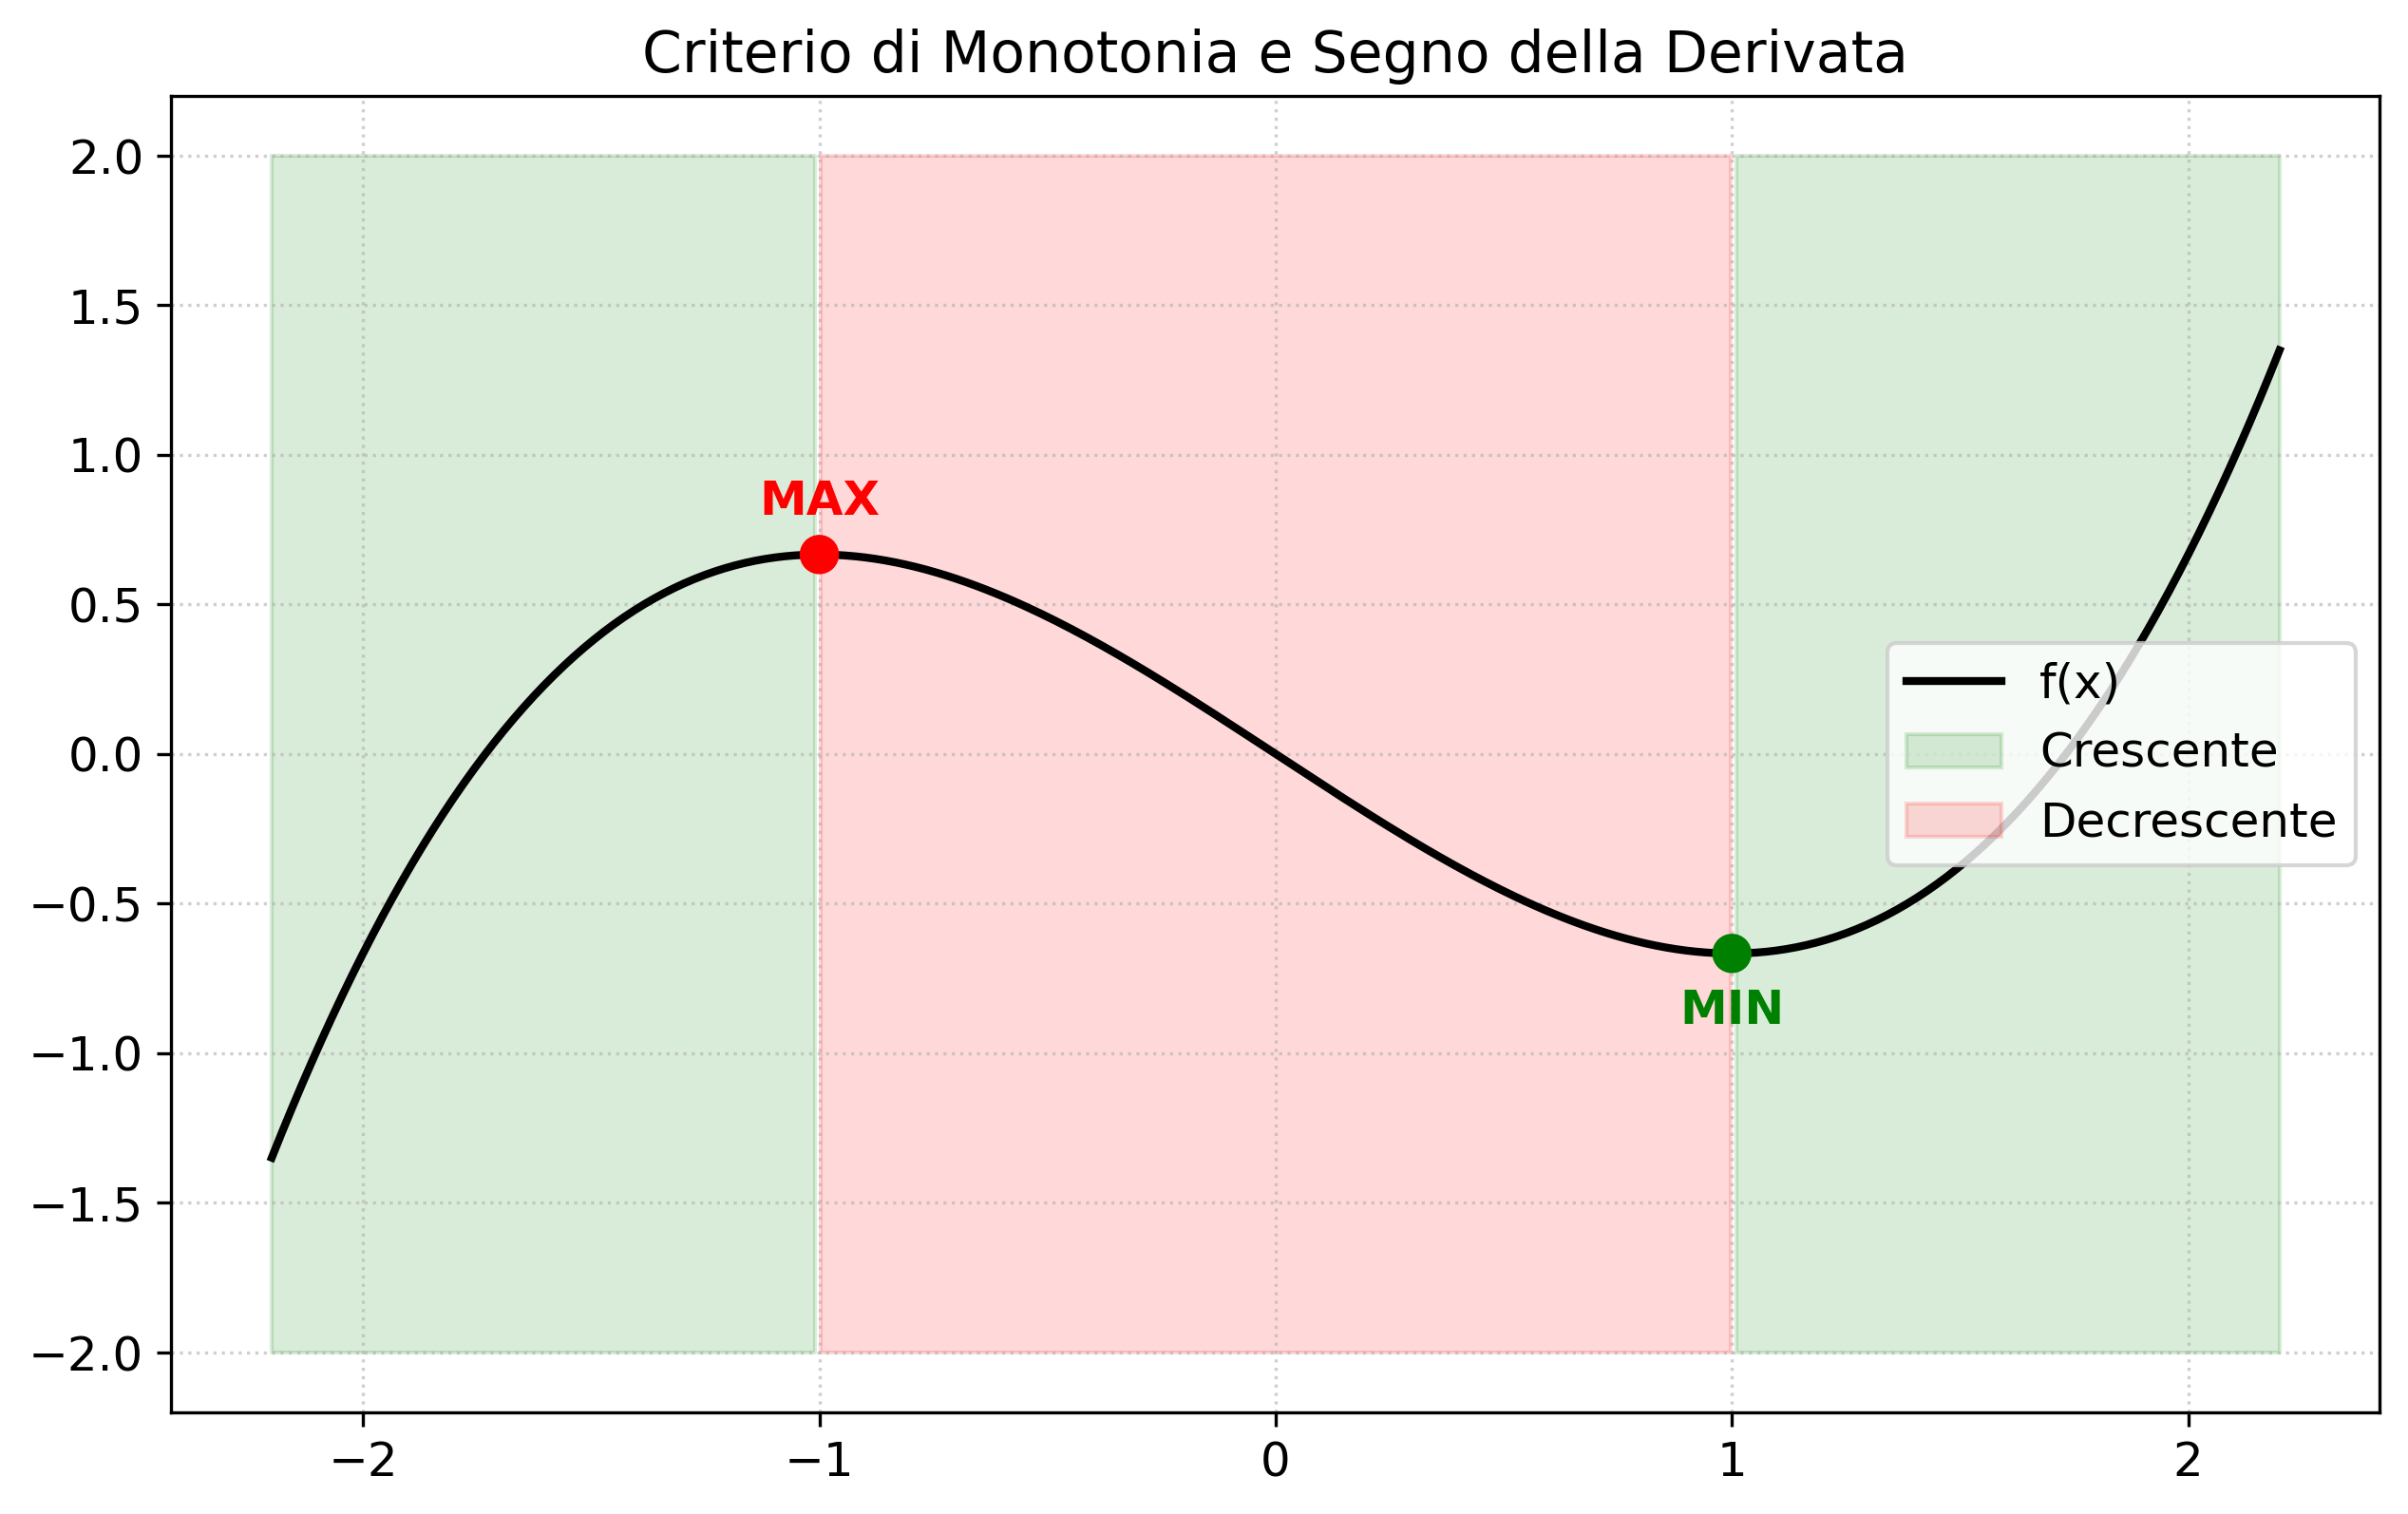
\includegraphics[width=0.7\textwidth]{img/monotonia_estremi.png}
    \end{center}
}

\pf{
    \begin{itemize}
        \item ($\implies$)
        \[ f'(x_{0})=\lim_{ h \to 0 } \frac{f(x_{0}+h)-f(x_{0})}{h}=\begin{dcases}
        h\to 0^+ \implies \frac{(+)}{(+)}\geq 0 \\
        h\to 0^- \implies \frac{(-)}{(-)}\geq 0 \\
        \end{dcases} \]
        \item ($\impliedby$) Hp $f'(x)\geq 0 \implies f \nearrow$.
        Siano $x_{1}<x_{2}$ e devo dimostrare che $f(x_{1})<f(x_{2})$.
        Applichiamo Lagrange in $[x_{1},x_{2}]\subseteq[a,b]$
        \[ \exists c \in ]x_{1},x_{2}[:\frac{f(x_{2})-f(x_{1})}{x_{2}-x_{1}}=f'(c)\geq 0 \]
    \end{itemize}
}

\subsection{Teorema di Caratterizzazione delle Funzioni Strettamente Monotone}

\thm{Caratterizzazione delle Funzioni Strettamente Monotone}{
    Sia $f:[a,b]\to \mathbb{R}$ continua.
    Sia $f$ derivabile in $]a,b[$.
    Allora: 
    \begin{enumerate}
        \item \[ f \nearrow_{S}\iff \begin{dcases}
        f'(x)\geq 0 \; \forall x \in ]a,b[ \\
        f' \text{ non si annulla in nessun sottointervallo in maniera costante}\\ \not \exists [c,d]\subseteq[a,b] : f' (x)=0 \; \forall x \in[c,d]
        \end{dcases} \] 
        \item \[ f \searrow_{S}\iff \begin{dcases}
        f'(x)\leq 0 \; \forall x \in ]a,b[ \\
        f' \text{ non si annulla in nessun sottointervallo in maniera costante}\\ \not \exists [c,d]\subseteq[a,b] : f' (x)=0 \; \forall x \in[c,d]
        \end{dcases} \]
    \end{enumerate}
}

\subsection{Condizione Sufficiente al Primo Ordine per gli Estremi Relativi}

\thm{Condizione Sufficiente al $1^{\circ}$ Ordine per gli Estremi Relativi}{
    Sia $f:[a,b]\to \mathbb{R}$ continua.
    Sia $f$ derivabile in $]a,b[$ escluso al più $x_{0}\in]a,b[$.
    Allora se:
    \begin{enumerate}
        \item \[ \begin{dcases}
        f'(x)\leq 0 \quad x <x_{0} \\
        f'(x)\geq 0 \quad x>x_{0}
        \end{dcases}\implies x_{0} \text{ è punto di \textit{Minimo relativo}} \]
        \item \[ \begin{dcases}
        f'(x)\geq 0 \quad x <x_{0} \\
        f'(x)\leq 0 \quad x>x_{0}
        \end{dcases}\implies x_{0} \text{ è punto di \textit{Massimo relativo}} \]
    \end{enumerate}
    \begin{center}
        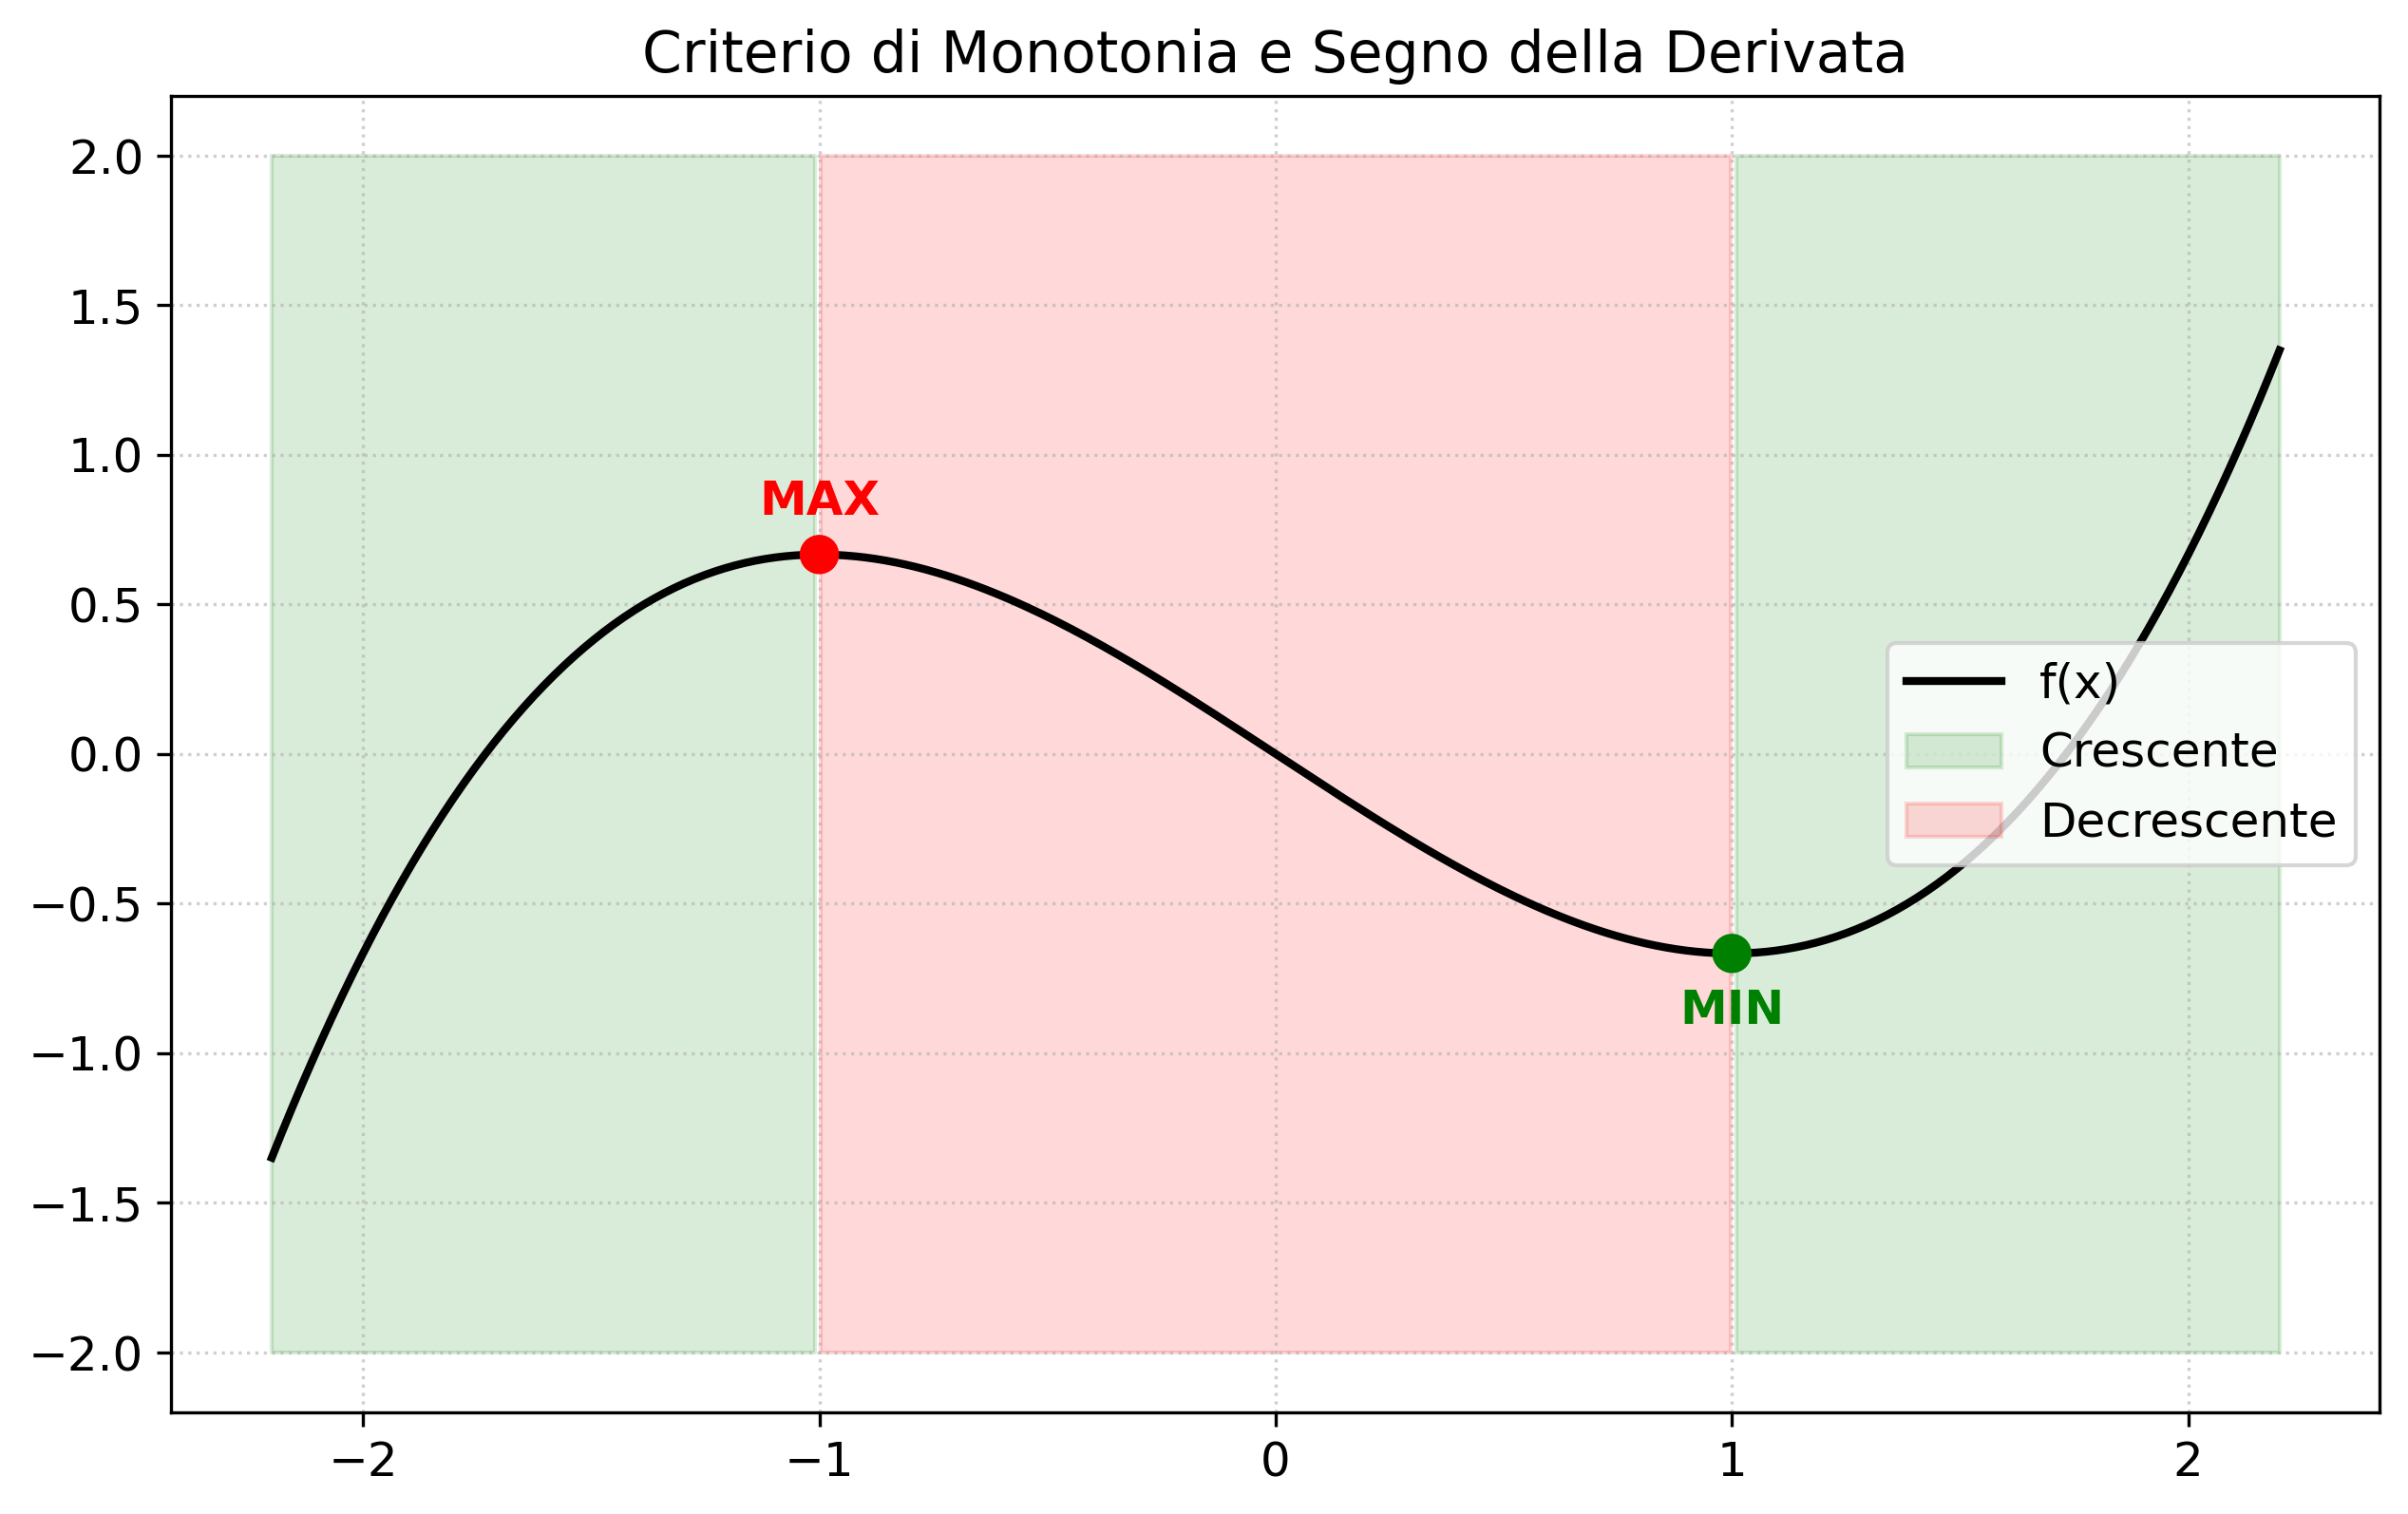
\includegraphics[width=0.7\textwidth]{img/monotonia_estremi.png}
    \end{center}
}

\subsection{Teoremi di de l'Hôpital}

\thm{1° Teorema di de l'Hôpital}{
    Siano $f,g$ derivabili in $]a,x_{0}[$ (con $x_{0}=+\infty$ eventualmente). Supponiamo che:
    \begin{enumerate}
        \item $\displaystyle \lim_{ x \to x_{0} } f(x)=\lim_{ x \to x_{0} } g(x)=0$
        \item $g'(x)\neq 0 \; \forall x \in ]a,x_{0}[$
        \item $\exists \lim_{ x \to x_{0} } \frac{f'(x)}{g'(x)}$
    \end{enumerate}
    Allora:
    \[ \lim_{ x \to x_{0} } \frac{f(x)}{g(x)}=\lim_{ x \to x_{0} } \frac{f'(x)}{g'(x)} \]
}

\ex{
    Esempio Utilizzo SBAGLIATO del Teo
    \begin{align*}
    & x_{0}=0\\
    &f(x)=x^2 \cos \frac{1}{x}\\
    & g(x)=e^x-1\to 0\\
    & \lim_{ x \to 0 } \frac{f'(x)}{g'(x)}=\lim_{ x \to 0 } \frac{2x \cos \frac{1}{x}+ \sin \frac{1}{x}}{e^x}= \not \exists \\
    & \lim_{ x \to 0 } \frac{f(x)}{g(x)}=0 
    \end{align*}
}

\pf{
    \begin{enumerate}
        \item Suppongo $x_{0} \in \mathbb{R}$ e usando la 1) prolungo $f,g$ in $x_{0}$.
        \item Osserviamo che $g(x)\neq 0\; \forall x \in ]a,x_{0}[$ perchè altrimenti Rolle andrebbe in contrasto con la 2) (delle hp).
        \item Sia $x_{n}\in]a, x_{0}[ \;\forall n$ e $x_{n}\to x_{0}$ e poniamo:
        \[ h(t)=f(t)g(x_{n})-g(t)f(x_{n}) \quad t \in]a,x_{0}[ \]
        Applico Rolle ad $h(t)$ in $[x_{n},x_{0}]$:
        \begin{itemize}
            \item $h(x_{n})=0$
            \item $h(x_{0})=0\implies \exists c_{n} \in ]x_{n}, x_{0}[:$
            \[ h'(c_{n})=0\implies 0=f'(c_{n})g(x_{n})-g'(c_{n})f(x_{n})\implies \frac{f'(c_{n})}{g'(c_{n})}=\frac{f(x_{n})}{g(x_{n})} \]
        \end{itemize}
    \end{enumerate}
}

\thm{2° Teorema di de l'Hôpital}{
    Se nella 1) del Teo di prima sostituiamo la seguente:
    \begin{itemize}
        \item[1b)] $\lim_{ x \to x_{0} } |f(x)|=\lim_{ x \to x_{0} } |g(x)|=+\infty$
        \item[2b)] ...
        \item[3b)] ...
    \end{itemize}
    $\implies$ Vale la stessa Tesi.
}